%% fcup-thesis.tex -- document template for PhD theses at FCUP
%%
%% Copyright (c) 2015 João Faria <joao.faria@astro.up.pt>
%%
%% This work may be distributed and/or modified under the conditions of
%% the LaTeX Project Public License, either version 1.3c of this license
%% or (at your option) any later version.
%% The latest version of this license is in
%%     http://www.latex-project.org/lppl.txt
%% and version 1.3c or later is part of all distributions of LaTeX
%% version 2005/12/01 or later.
%%
%% This work has the LPPL maintenance status "maintained".
%%
%% The Current Maintainer of this work is
%% João Faria <joao.faria@astro.up.pt>.
%%
%% This work consists of the files listed in the accompanying README.

%% SUMMARY OF FEATURES:
%%
%% All environments, commands, and options provided by the `ut-thesis'
%% class will be described below, at the point where they should appear
%% in the document.  See the file `ut-thesis.cls' for more details.
%%
%% To explicitly set the pagestyle of any blank page inserted with
%% \cleardoublepage, use one of \clearemptydoublepage,
%% \clearplaindoublepage, \clearthesisdoublepage, or
%% \clearstandarddoublepage (to use the style currently in effect).
%%
%% For single-spaced quotes or quotations, use the `longquote' and
%% `longquotation' environments.


%%%%%%%%%%%%         PREAMBLE         %%%%%%%%%%%%

%%  - Default settings format a final copy (single-sided, normal
%%    margins, one-and-a-half-spaced with single-spaced notes).
%%  - For a rough copy (double-sided, normal margins, double-spaced,
%%    with the word "DRAFT" printed at each corner of every page), use
%%    the `draft' option.
%%  - The default global line spacing can be changed with one of the
%%    options `singlespaced', `onehalfspaced', or `doublespaced'.
%%  - Footnotes and marginal notes are all single-spaced by default, but
%%    can be made to have the same spacing as the rest of the document
%%    by using the option `standardspacednotes'.
%%  - The size of the margins can be changed with one of the options:
%%     . `narrowmargins' (1 1/4" left, 3/4" others),
%%     . `normalmargins' (1 1/4" left, 1" others),
%%     . `widemargins' (1 1/4" all),
%%     . `extrawidemargins' (1 1/2" all).
%%  - The pagestyle of "cleared" pages (empty pages inserted in
%%    two-sided documents to put the next page on the right-hand side)
%%    can be set with one of the options `cleardoublepagestyleempty',
%%    `cleardoublepagestyleplain', or `cleardoublepagestylestandard'.
%%  - Any other standard option for the `report' document arclass can be
%%    used to override the default or draft settings (such as `10pt',
%%    `11pt', `12pt'), and standard LaTeX packages can be used to
%%    further customize the layout and/or formatting of the document.

%% *** Add any desired options. ***
%PDF
%\documentclass[a4paper,narrowmargins,12pt,oneside,draft,onehalfspaced,singlespacednotes]{fcup-thesis}
%\documentclass[a4paper,narrowmargins,12pt,oneside,onehalfspaced,singlespacednotes]{fcup-thesis}
%Print
%\documentclass[draft,a4paper,narrowmargins,12pt,twoside,openright,onehalfspaced,singlespacednotes]{fcup-thesis}
\documentclass[a4paper,narrowmargins,12pt,twoside,openright,onehalfspaced,singlespacednotes]{fcup-thesis}

%% *** Add \usepackage declarations here. ***
%% The standard packages `geometry' and `setspace' are already loaded by
%% `ut-thesis' -- see their documentation for details of the features
%% they provide.  In particular, you may use the \geometry command here
%% to adjust the margins if none of the ut-thesis options are suitable
%% (see the `geometry' package for details).  You may also use the
%% \setstretch command to set the line spacing to a value other than
%% single, one-and-a-half, or double spaced (see the `setspace' package
%% for details).
% Overfull statements
\pretolerance=150
\setlength{\emergencystretch}{3em}
% Overfull end
\usepackage[english]{babel}
\usepackage{lipsum}
\usepackage[utf8]{inputenc}


%%% Additional useful packages
%%% ----------------------------------------------------------------
\usepackage{array}
\usepackage{amsmath}  
\usepackage{amssymb}
\usepackage{amsfonts}
\DeclareFontFamily{OT1}{pzc}{}
\DeclareFontShape{OT1}{pzc}{m}{it}{<-> s * [0.900] pzcmi7t}{}
\DeclareMathAlphabet{\mathpzc}{OT1}{pzc}{m}{it}
\usepackage{amsthm}      
\usepackage[ruled,algochapter]{algorithm2e}
\usepackage{algorithmic}
\usepackage{bm}
\usepackage[mathscr]{euscript}
\usepackage{graphicx}       
\usepackage{psfrag}         
\usepackage{fancyvrb}    
\usepackage{float}
\usepackage{ltablex}
\usepackage[square,sort,comma,numbers]{natbib}        
\usepackage{bbding}         
\usepackage{dcolumn}        
\usepackage{booktabs} 
\usepackage{multirow}
\usepackage{paralist}     
\usepackage{ifdraft}  
\usepackage{indentfirst}    
\usepackage[nottoc,notlof,notlot]{tocbibind}
\usepackage{url}
\usepackage{tabularx}
\usepackage{subcaption}
\usepackage[unicode]{hyperref}
\usepackage{xcolor}

\hypersetup{pdftitle=LiDAR obstacle detection and avoidance, 
            pdfauthor=Alojz Gomola,
            colorlinks=false,
            urlcolor=blue,
            pdfstartview=FitH,
            pdfpagemode=UseOutlines,
            pdfnewwindow,
            breaklinks
          }
\usepackage{array}
\newcolumntype{L}[1]{>{\raggedright\let\newline\\\arraybackslash\hspace{0pt}}m{#1}}
\newcolumntype{C}[1]{>{\centering\let\newline\\\arraybackslash\hspace{0pt}}m{#1}}
\newcolumntype{R}[1]{>{\raggedleft\let\newline\\\arraybackslash\hspace{0pt}}m{#1}}         
\newcolumntype{B}{X}
\newcolumntype{S}[1]{>{\hsize=#1\textwidth}X}

\newcommand{\FIGDIR}{./Pics}    %%% directory containing figures
\newcommand{\twolinecellr}[2][r]{%
  \begin{tabular}[#1]{@{}r@{}}#2\end{tabular}}
\newcommand{\secState}[1]{
	\ifdraft{(#1) }{}
}
\theoremstyle{plain}
\newtheorem{theorem}{Theorem}
\newtheorem{lemma}[theorem]{Lemma}
\newtheorem{proposition}[theorem]{Proposition}

\theoremstyle{plain}
\newtheorem{definition}{Definition}
\newtheorem{problem}{Problem}
\newtheorem{example}{Example}
\newtheorem{assumption}{Assumption}

\theoremstyle{remark}
\newtheorem*{corollary}{Corollary}
\newtheorem*{note}{Note}




\newenvironment{dokaz}{
  \par\medskip\noindent
  \textit{Proof}.
}{
\newline
\rightline{\SquareCastShadowBottomRight}
}

\newenvironment{constraints}[1]{
  \par\medskip\noindent
  \textit{Constraints #1} \\
}{
\newline
\rightline{\SquareCastShadowBottomRight}
}


%\bibliographystyle{plainnat}     %% Author (year) style
\bibliographystyle{unsrt}        %% [number] style
\setcitestyle{square}

% Section  3.7 Challenge list
\newif\ifproblemchallenge   %# Build block for problem challenges
\problemchallengetrue       %# Show comments

\newcommand{\R}{\mathbb{R}}
\newcommand{\N}{\mathbb{N}}

\DeclareMathOperator{\pr}{\textsf{P}}
\DeclareMathOperator{\E}{\textsf{E}\,}
\DeclareMathOperator{\var}{\textrm{var}}
\DeclareMathOperator{\sd}{\textrm{sd}}


\newcommand{\T}[1]{#1^\top}        

\newcommand{\goto}{\rightarrow}
\newcommand{\gotop}{\stackrel{P}{\longrightarrow}}
\newcommand{\maon}[1]{o(n^{#1})}
\newcommand{\abs}[1]{\left|{#1}\right|}
\newcommand{\dint}{\int_0^\tau\!\!\int_0^\tau}
\newcommand{\isqr}[1]{\frac{1}{\sqrt{#1}}}
\newcommand{\norm}[1]{\left\lVert#1\right\rVert}


\newcommand{\pulrad}[1]{\raisebox{1.5ex}[0pt]{#1}}
\newcommand{\mc}[1]{\multicolumn{1}{c}{#1}}
\newcommand{\TBD}[1]{\color{red}\emph{--TBD:}#1\color{black}}

%%%%%%%%%%%%%%%%%%%%%%%%%%%%%%%%%%%%%%%%%%%%%%%%%%%%%%%%%%%%%%%%%%%%%%%%
%%                                                                    %%
%%                   ***   I M P O R T A N T   ***                    %%
%%                                                                    %%
%%  Fill in the following fields with the required information:       %%
%%   - \degree{...}       name of the degree obtained                 %%
%%   - \department{...}   name of the graduate department             %%
%%   - \gradyear{...}     year of graduation                          %%
%%   - \author{...}       name of the author                          %%
%%   - \title{...}        title of the thesis                         %%
%%%%%%%%%%%%%%%%%%%%%%%%%%%%%%%%%%%%%%%%%%%%%%%%%%%%%%%%%%%%%%%%%%%%%%%%

%% *** Change this example to appropriate values. ***
\degree{Doctor of Philosophy}
\department{Departamento de Matem\'{a}tica}
\gradyear{2019}
\author{Alojz Gomola}
\title{Obstacle Avoidance Framework based on Reach Sets}

%% *** NOTE ***
%% Put here all other formatting commands that belong in the preamble.
%% In particular, you should put all of your \newcommand's,
%% \newenvironment's, \newtheorem's, etc. (in other words, all the
%% global definitions that you will need throughout your thesis) in a
%% separate file and use "\input{filename}" to input it here.


%% *** Adjust the following settings as desired. ***

%% List only down to subsections in the table of contents;
%% 0=chapter, 1=section, 2=subsection, 3=subsubsection, etc.
\setcounter{tocdepth}{3}

%% Make each page fill up the entire page.
\flushbottom


%%%%%%%%%%%%      MAIN  DOCUMENT      %%%%%%%%%%%%

\begin{document}


%%%%%%%%%%%%%%%%%%%%%%%%%%%%%%%%%%%%%%%%%%%%%%%%%%%%%%%%%%%%%%%%%%%%%%%%
%%  Put your Chapters here; the easiest way to do this is to keep     %%
%%  each chapter in a separate file and `\include' all the files.     %%
%%  Each chapter file should start with "\chapter{ChapterName}".      %%
%%  Note that using `\include' instead of `\input' will make each     %%
%%  chapter start on a new page, and allow you to format only parts   %%
%%  of your thesis at a time by using `\includeonly'.                 %%
%%%%%%%%%%%%%%%%%%%%%%%%%%%%%%%%%%%%%%%%%%%%%%%%%%%%%%%%%%%%%%%%%%%%%%%%

%% *** Include chapter files here. ***

\setcounter{chapter}{6}
\setcounter{section}{6}

    %06-07 Avoidance Concept	
    \section{\secState{R}Avoidance Concept}\label{s:avoidanceConcept}
This section introduces \emph{Platform Independent Avoidance Concept} core functionality (fig. \ref{fig:AvoidanceFrameworkConceptNew}) modules responsible for \emph{path finding} and \emph{navigation} including \emph{data fusion} interface. The sections are organized like follow:

\begin{enumerate}
    \item \emph{Data Fusion} (sec. \ref{s:sensorFusion}) - implementation details of \emph{input interface} responsible for \emph{processing partial known world data} into final visibility, obstacle, intruder, and, constraints ratings.
    
    \item \emph{Avoidance Grid Run} (sec.\ref{s:aviudabceGridRun}) (inner avoidance run) - the \emph{best path finding} in one \emph{Avoidance Grid} with \emph{situation assessment} done.
    
    \item \emph{Mission Control Run} (sec . \ref{s:missionControlRun}) (outer navigation run) - main navigation and decision making algorithm for \emph{non-cooperative obstacle avoidance}.
    
    \item \emph{Computation Complexity} (sec. \ref{sec:MCRcomputationalComplexity}) - the \emph{computational feasibility study} and \emph{weak point identification} of our approach.
    
    \item \emph{Safety Margin Calculation} (sec. \ref{s:safetyMarginCalculation}) - the boundaries of \emph{Safety Margin} and identified \emph{impact factors}.
\end{enumerate}

    	\subsection{Data fusion}\label{s:sensorFusion}

\paragraph{Summary:} There is a need for the final threat assessment in the Avoidance Grid. The data fusion provides mechanisms to represent, process, and assess threat in the cell including the safety of trajectories in the RSA. The output of the data fusion procedure is used further in Avoidance run (sec. \ref{s:aviudabceGridRun}).


\paragraph{Introduction:} The data fusion interfaces \emph{Sensor Field} and \emph{Information Sources} from \emph{cell/trajectory properties}. The \emph{Data Fusion Function} is outlined in (\ref{eq:DataFusionFunction}). 

First, there will be an outline of \emph{Partial Rating} commutation. Then these ratings will be discredited into Boolean values as properties of \emph{Avoidance Grid/Trajectory}. Then these Boolean values will be used for further classification of  space into \emph{Free(t), Occupied(t), Restricted(t)} and \emph{Uncertain(t)}.

All mentioned ratings are the result of \emph{Filtered Sensor Readings} from \emph{Sensor Field} and \emph{Information Sources} with prior processing. This section will focus on \emph{final fuzzy value calculation} and \emph{discretization}. 
\begin{note}
    All rating values are in the \emph{range:} $[0,1]$, and they were introduced in previous sections.
\end{note}


\paragraph{Visibility:} The \emph{sensor reading} of \emph{sensor} if \emph{Sensor field} returns a value of \emph{visibility} for cell space in time of decision $t_i$.

The \emph{visibility} for the cell is given in (eq. \ref{eq:visibilityForCell}) as minimal visibility calculated from all capable sensors in \emph{Sensor Field}.

\begin{equation}\label{eq:visibilityForCell}
    visibility(cell_{i,j,k}) = \min \left\{\begin{aligned}visibility(cell_{i,j,k},&sensor_i):\\&\forall sensor_i \in Sensor Field\end{aligned}\right\}
\end{equation}

\noindent The example of \emph{visibility} calculation for \emph{LiDAR} sensor is given in (fig. \ref{fig:mapObstacleStatesAfterDataFusion}).

\begin{note}
    Sensor reliability for \emph{visibility} is already accounted for prior \emph{data fusion}. If not \emph{weighted average} should be used instead. 
\end{note}

\paragraph{Detected Obstacle:} Sensors detect the physical obstacles  in \emph{Sensor Field}. Each \emph{sensor} returns \emph{detected obstacle rating} in the range $[0,1]$ reflecting the probability of obstacle occurrence in a given  cell.

The \emph{maximal value} of \emph{detected obstacle} rating is selected from readings multiplied by \emph{visibility rating} to enforce \emph{visibility bias}.

\begin{multline}\label{eq:detectedObstacleRatingForCell}
    obstacle(cell_{i,j,k}) = \max \left\{\begin{aligned}obstacle(cell_{i,j,k},&sensor_i):\\&\forall sensor_i \in SensorField\end{aligned}\right\}\times\dots\\\dots\times visibility(cell_{i,j,k})
\end{multline}

\noindent The example of \emph{detected obstacle rating} calculation for \emph{LiDAR} sensor is given in (eq. \ref{eq:naiveObstacleRate}).

\paragraph{Map Obstacle:} The \emph{Information Sources} are feeding \emph{Avoidance Grid} with partial information of \emph{Map obstacle rating}. \emph{Map Obstacle Rating} shows the certainty that \emph{charted obstacle} is in a given cell. This property is bound to \emph{Information Source}, and it has the \emph{range} in  $[0,1]$.

The \emph{Map Obstacle Rating} for a cell (eq. \ref{eq:mapObstacleRatingForCell}) is calculated as the product of maximal \emph{Map Obstacle Rating} and \emph{inverse visibility}. This gives \emph{visibility biased} certainty of \emph{Map Obstacle}.

\begin{multline}\label{eq:mapObstacleRatingForCell}
    map(cell_{i,j,k}) = \max 
    \left\{\begin{aligned}map(&cell_{i,j,k},source_i):\\&\forall source_i \in InformationSources\end{aligned}\right\}\times\dots\\\dots\times \left(1-visibility(cell_{i,j,k})\right)
\end{multline}

\noindent The example of \emph{Map Obstacle Rating} calculation is given in (fig. \ref{fig:mapObstacleStatesAfterDataFusion}).


\paragraph{Intruder:} There is a set of \emph{Active Intruders}, each intruder is using its \emph{parametric intersection model}. This parametric \emph{intersection} model calculates \emph{partial intersection ratings} representing \emph{intersection certainty} ranging in $[0,1]$. The more \emph{partial intersection rating} is closer to 1 the higher is the probability of aerial collision with that intruder in that cell. 

The \emph{geometrical bias} is used for cumulative of multiple intruders; the \emph{intruders are not cooperative}; therefore their occurrence cannot be addressed by the simple \emph{maximum}. The proposed formula (eq. \ref{eq:intruderRatingForCell}) is simply bypassing the intruder rating if there is one intruder. If there  are more intruders, the geometrical bias is applied.


\begin{equation}\label{eq:intruderRatingForCell}
    intruder(cell_{i,j,k}) = 1 - \prod_{\forall intruder_i \in Intruders} \left(1- intersection\left(\begin{gathered}cell_{i,j,k},\\intruder_i\end{gathered}\right)\right)
\end{equation}

\noindent The \emph{intruder intersection models} are outlined in (app. \ref{app:IntruderProbabilisticModels}). 

\paragraph{Constraint:} The \emph{constraints} are coming from various \emph{Information Sources}, the \emph{hierarchical constraint application} is resolved by higher level logic. All \emph{constraints} in this context are considered as \emph{hard}.

The \emph{Constraints rating} (eq. \ref{eq:constraintRatingForCell}) is in the \emph{range} $[0,1]$ reflecting certainty of constraint application in the cell (usually 1).

\begin{equation}\label{eq:constraintRatingForCell}
    constraint(cell_{i,j,k}) = \max \left\{\begin{aligned}constraint(&cell_{i,j,k},source_i):\\&\forall source_i \in InformationSources\end{aligned}\right\}
\end{equation}

\noindent The \emph{Constraint Rating} calculation example for \emph{static} constraints is given in (sec. \ref{s:virtualConstraints}), the example for \emph{moving} constraints is given by (def. \ref{def:movingConstraint}).

\begin{note}{Weather}
    is already considered in constraints; the weather is handled as soft/hard static/moving constraints.
\end{note}

\paragraph{Threat:} The concept of threat is a \emph{rating of expected harm} to receive in a given portion of space. The threat can be time-bound to \emph{decision time $t_i$} (time sensitive \emph{intruder intersection models}).

The \emph{harm prioritization} is addressed by higher navigation logic (fig. \ref{fig:missionControlRunActivityDiagram}). All \emph{sources of harm} are considered as equal. The threat is formalized in the \emph{following definition}:

\begin{definition}{The Threat}\label{def:threat} is considered as any source of harm. The threat is a \emph{maximal aggregation} of various harm ratings. Our \emph{threat} for a  specific cell is defined by (eq. \ref{eq:threatRatingForCell}).
    \begin{equation}\label{eq:threatRatingForCell}
        threat(cell_{i,j,k}) = \max\left\{\begin{gathered}obstacle(cell_{i,j,k}),map(cell_{i,j,k}),\\intruder(cell_{i,j,k}),constraint(cell_{i,j,k})\end{gathered}\right\}
    \end{equation}
\end{definition}

\paragraph{Reachability:} The \emph{Reachability} for trajectory reflects how safe is the \emph{path along}. The \emph{Threat} (def. \ref{def:threat}) for each cell has been already assessed.  The set of \emph{Passing Cells} is defined in \emph{Trajectory Footprint} (eq. \ref{eq:setOfPassedCells}).

The \emph{Trajectory Reachability} is given as a product of \emph{Threats} along the trajectory (eq. \ref{eq:trajectoryReachibility}). The \emph{Trajectory Reachability} can be calculated for each \emph{trajectory segment} given as $\{movement_1,\dots,movement_i\}$ $\subset$ $Buffer$ originating from $state_0$.


\begin{equation}\label{eq:trajectoryReachibility}
    reachibility(Trajectory) = \prod_{Passing Cells}^{\forall cell_{i,j,k}\in} \left(1- threat(c_{i,j,k})\right)
\end{equation}

\begin{note}
    The \emph{Reachability} of \emph{trajectory} segment gives the property of \emph{safety} of route from the beginning, until the last point of the segment. There can be a very unsafe trajectory which is very safe from the beginning.
\end{note}


The \emph{Reachability} of the \emph{cell} is given by the best trajectory segment passing through the \emph{given cell}. This is given by property, that every trajectory is originating from root $state_0$, which means that one safe route is sufficient to reach space in the cell.

\newpage
The \emph{Trajectory segment} reachability is sufficient, because the overall performance is not interesting, the \emph{local reachability} is sufficient. The cell reachibility is formally defined in (eq. \ref{eq:cellReachibility}).

\begin{multline}\label{eq:cellReachibility}
    reachability(cell_{i,j,k}) = \max\{Trajectory.Segment(cell_{i,j,k}). Reachability: \\\forall Trajectory \in Passing Trajectories (cell{i,j,k})\}
\end{multline}
    
\begin{note}
    Function Trajectory.Segment($cell_{i,j,k}$). Reachability gives same results for any segment in $cell_{i,j,k}$, because (eq. \ref{eq:trajectoryReachibility}) accounts each cell $threat$ only once.
\end{note}

\paragraph{Discretization:} The \emph{fault tolerant} implementation needs to implement sharp Boolean values of properties mentioned before. The \emph{fuzzy values} are usually threshold to Boolean equivalent. The \emph{operational standards} for \emph{Manned Aviation} \cite{icao4444} demands the fail rate below $10^{-7}$ because there is no definition for \emph{UAS} the \emph{minimal fail rate} is expected to be at a similar level.

The \emph{fuzzy values} $[0,1]$ are projected to \emph{Boolean} properties of \emph{cell} and \emph{Trajectory} in the following manner (tab. \ref{tab:defuzificationRatings}).


The high values of \emph{Visibility} (eq. \ref{eq:visibilityForCell}) and \emph{Reachability} (eq. \ref{eq:cellReachibility}, \ref{eq:trajectoryReachibility}) are expected. The low \emph{threshold} for \emph{threats} values is expected. The error margin is solved by \emph{Sensor Fusion}, therefore, initial \emph{false positive} cases have a low rate. The \emph{Detected Obstacle Rate} (eq. \ref{eq:detectedObstacleRatingForCell}), \emph{Map Obstacle Rate} (eq. \ref{eq:mapObstacleRatingForCell}), \emph{Intruder Rate} (eq. \ref{eq:intruderRatingForCell}), and \emph{Constraint Rate} (eq. \ref{eq:constraintRatingForCell}) thresholds are considered low.

\begin{table}[H]
    \centering
    \begin{tabular}{c|ccc}
        \multicolumn{4}{c}{Threshold = $10^{-7}$}\\\hline\hline
        Visibile & $visibility(cell_{i,j,k})$&$\ge$&$(1-threshold)$ \\\hline
        Detected Obstacle &  $obstacle(cell_{i,j,k}) $&$ \ge $&$ threshold$\\\hline
        Map Obstacle &  $map(cell_{i,j,k})$&$\ge$&$threshold$\\\hline
        Intruder &  $intruder(cell_{i,j,k})$&$\ge$&$threshold$\\\hline
        Constraint &  $constraint(cell_{i,j,k})$&$\ge$&$threshold$\\\hline\hline
        Reachable Trajectory &  $reachability(trajectory)$&$\ge$&$(1-threshold)$\\\hline
        Reachable Cell &  $reachibility(cell_{i,j,k})$&$\ge$&$(1-threshold)$
    \end{tabular}
    \caption{Changing ratings from fuzzy to Boolean parameters.}
    \label{tab:defuzificationRatings}
\end{table}

\newpage
\paragraph{Space Classification:} The \emph{Data Fusion Function} is outlined in (\ref{eq:DataFusionFunction}). This classification is resulting in four distinct cell sets.

The \emph{Uncertain} space for decision time $t_i$ is a portion of \emph{Avoidance Grid} which \emph{UAS} cannot \emph{read} with \emph{Sensor Field}. The \emph{cells} with a $\neg Visible$ property. The \emph{Uncertain} space is given by (eq. \ref{eq:UncertainDataFusion}).

\begin{equation}\label{eq:UncertainDataFusion}
    Uncertain(t_i) = \left\{cell_{i,j,k}:cell_{i,j,k}\in AvoidanceGrid(t_i),cell_{i,j,k}.\neg Visible \right\}
\end{equation}

\noindent The \emph{Occupied} space for decision time $t_i$ is the set of cells which are classified as \emph{Detected Obstacles}. The \emph{Visibility} is not an issue, due to the initial damping in (eq. \ref{eq:detectedObstacleRatingForCell}). The formal definition is the space portion where it is possible to detect \emph{obstacle bodies} or their portions (eq. \ref{eq:ocuupiedDataFusion}).

\begin{equation}\label{eq:ocuupiedDataFusion}
    Occupied(t_i) = \left\{cell_{i,j,k}:\begin{aligned}&cell_{i,j,k}\in AvoidanceGrid(t_i),\\&cell_{i,j,k}.DetectedObstacle\end{aligned}\right\}
\end{equation}

\noindent The \emph{Constrained} space for decision time $t_i$ is \emph{Visible} portion of \emph{Avoidance Grid} where the \emph{Intruder} or \emph{Constraint} is present. The mathematical formulation is given in (eq. \ref{eq:constrainedDataFusion}).

\begin{equation}\label{eq:constrainedDataFusion}
    Constrained(t_i) = \left\{cell_{i,j,k}:
    \begin{aligned}
        &cell_{i,j,k} \in AvoidanceGrid(t_i),\\
        &cell_{i,j,k}.Visible,\\
        &cell_{i,j,k}.Constraint \vee cell_{i,j,k}.Intruder
    \end{aligned}\right\}
\end{equation}

\noindent The \emph{Free} space is the space which is \emph{Visible} and $\neg Obstacle$,  $\neg Intruder$, and, $\neg Constrained$. The mathematical definition is simple set subtractions from \emph{Avoidance Grid} (eq. \ref{eq:freeDataFusion}).

\begin{multline}\label{eq:freeDataFusion}
    Free(t_i) = AvoidanceGrid(t_i) -\dots\\\dots -\left(Uncertain(t_i)\cup Occupied(t_i)\cup  Constrained(t_i)\right)
\end{multline}

\noindent The \emph{Reachable} space for time $t_i$, used in \emph{Avoidance} because its free and there is a safe trajectory, is given as a set of cells from \emph{Avoidance Grid} which are \emph{Reachable}. The mathematical definition is given in (eq. \ref{eq:ReachableDataFusion}).

\begin{equation}\label{eq:ReachableDataFusion}
    Reachable(t_i) = \left\{cell_{i,j,k}:\begin{aligned}&cell_{i,j,k}\in AvoidanceGrid(t_i),\\&cell_{i,j,k}.Reachable\end{aligned}\right\}
\end{equation}

\begin{note}{The Reachable Space at decision time $t_i$:} 
The \emph{Reachable space} is a non-empty set and its a subset of \emph{Free($t_i$)} space:    

\begin{equation}\label{eq:reachableDataFusionConstraints}
    |Reachable(t_i)| > 0, \quad Reachable(t_i) \subset Free(t)
\end{equation}
\end{note}

    	\newpage
\subsection{(R) Avoidance Grid Run}\label{s:aviudabceGridRun}
\paragraph{Main Goal:} The main goal of this section is to introduce the trajectory selection process, based on a \emph{situation assessment}, originating from \emph{Data Fusion Procedure} (sec. \ref{s:sensorFusion}). 

\begin{note}
    The \emph{rating calculation} is outlined in (sec. \ref{s:sensorFusion}). Low cost sensor fusion example usable to feed our data fusion procedure is given in \cite{sabatini2013low}. Semi-optimal concatenation trajectory search  like ours can be found in \cite{shaw1998using}.
\end{note}

\begin{figure}[H]
\centering
    \begin{subfigure}{0.48\textwidth}
        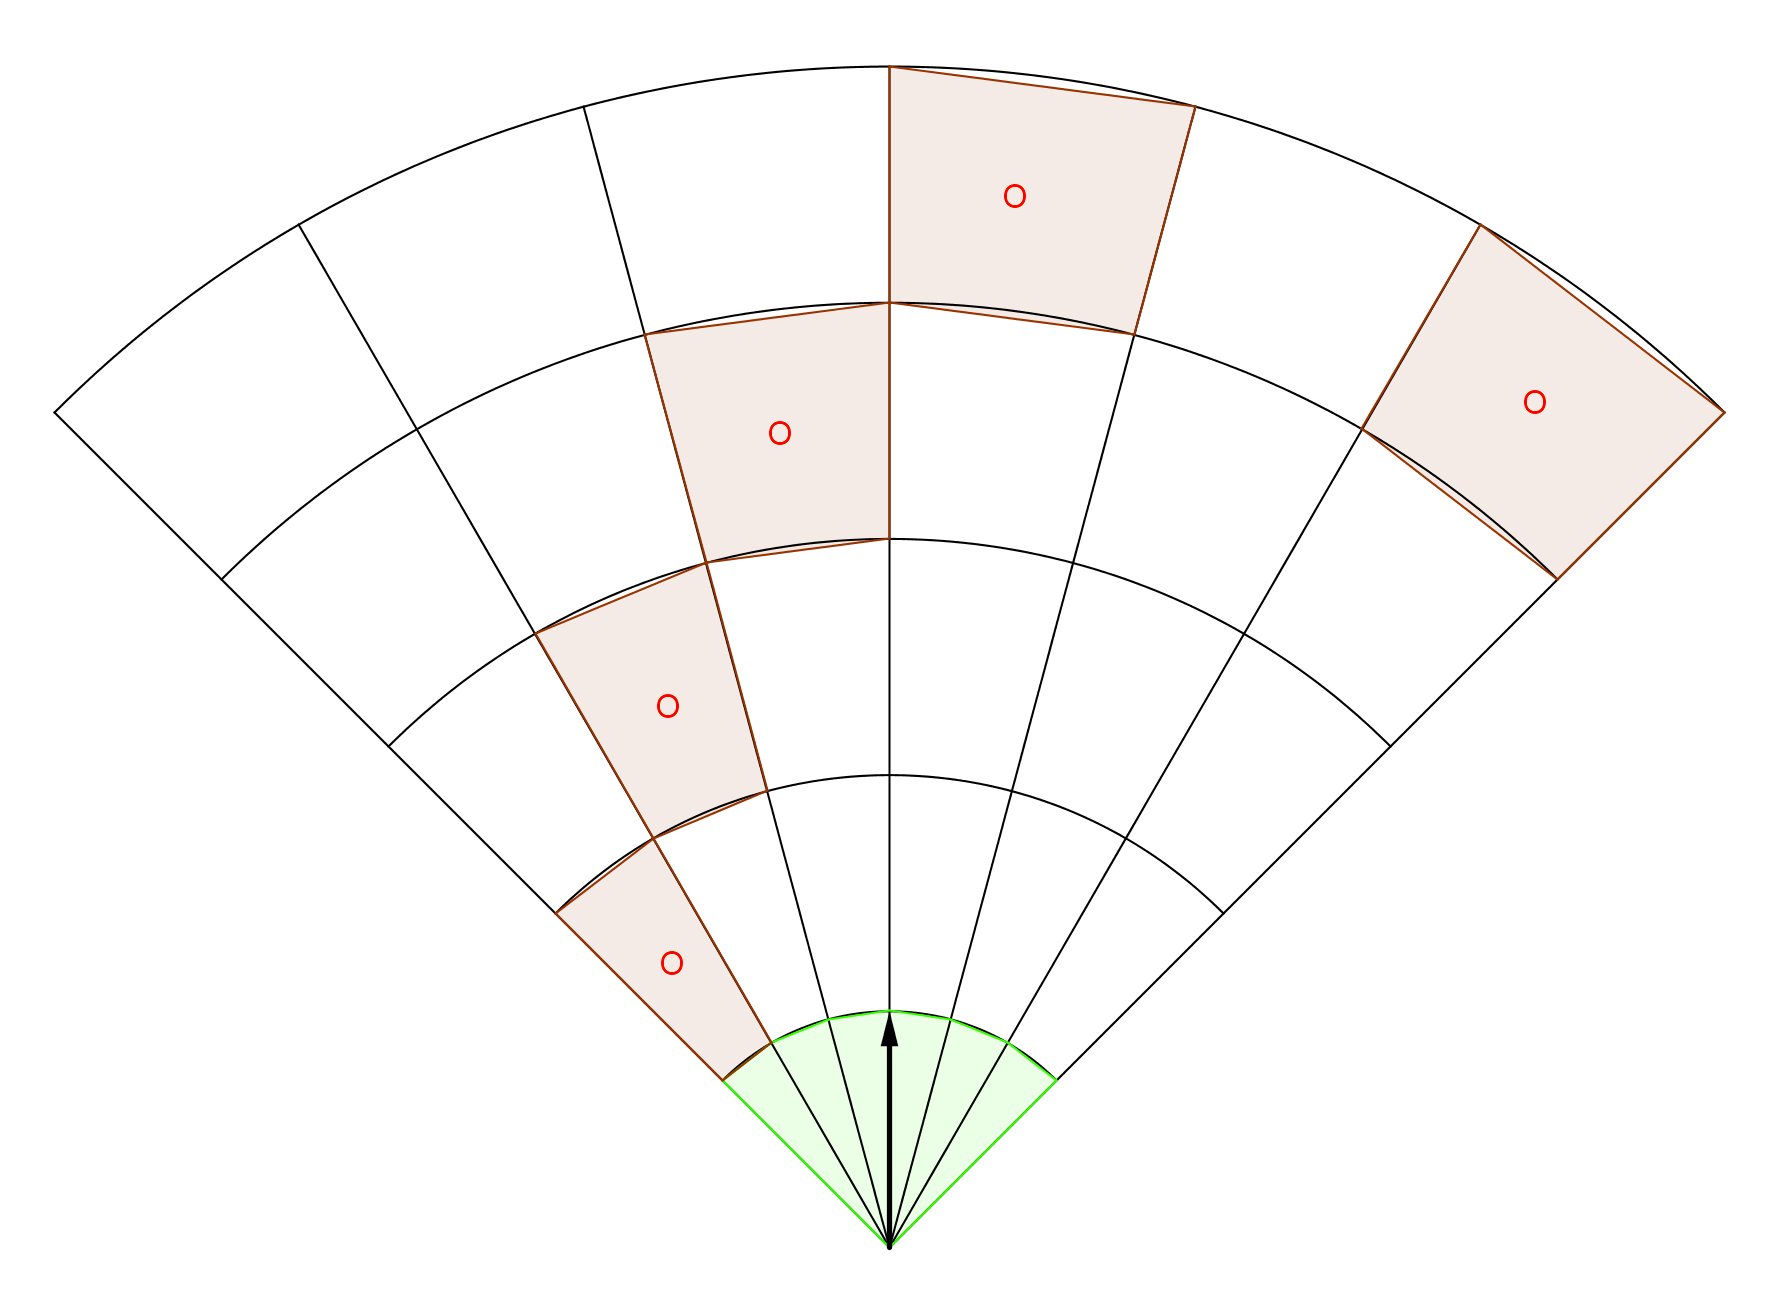
\includegraphics[width=0.9\linewidth]{\FIGDIR/CA001ObstacleDetection}
        \caption{Obstacle detection.}
        \label{fig:obstacleDetectionAvoidanceGrid}
    \end{subfigure}
    \begin{subfigure}{0.48\textwidth}
        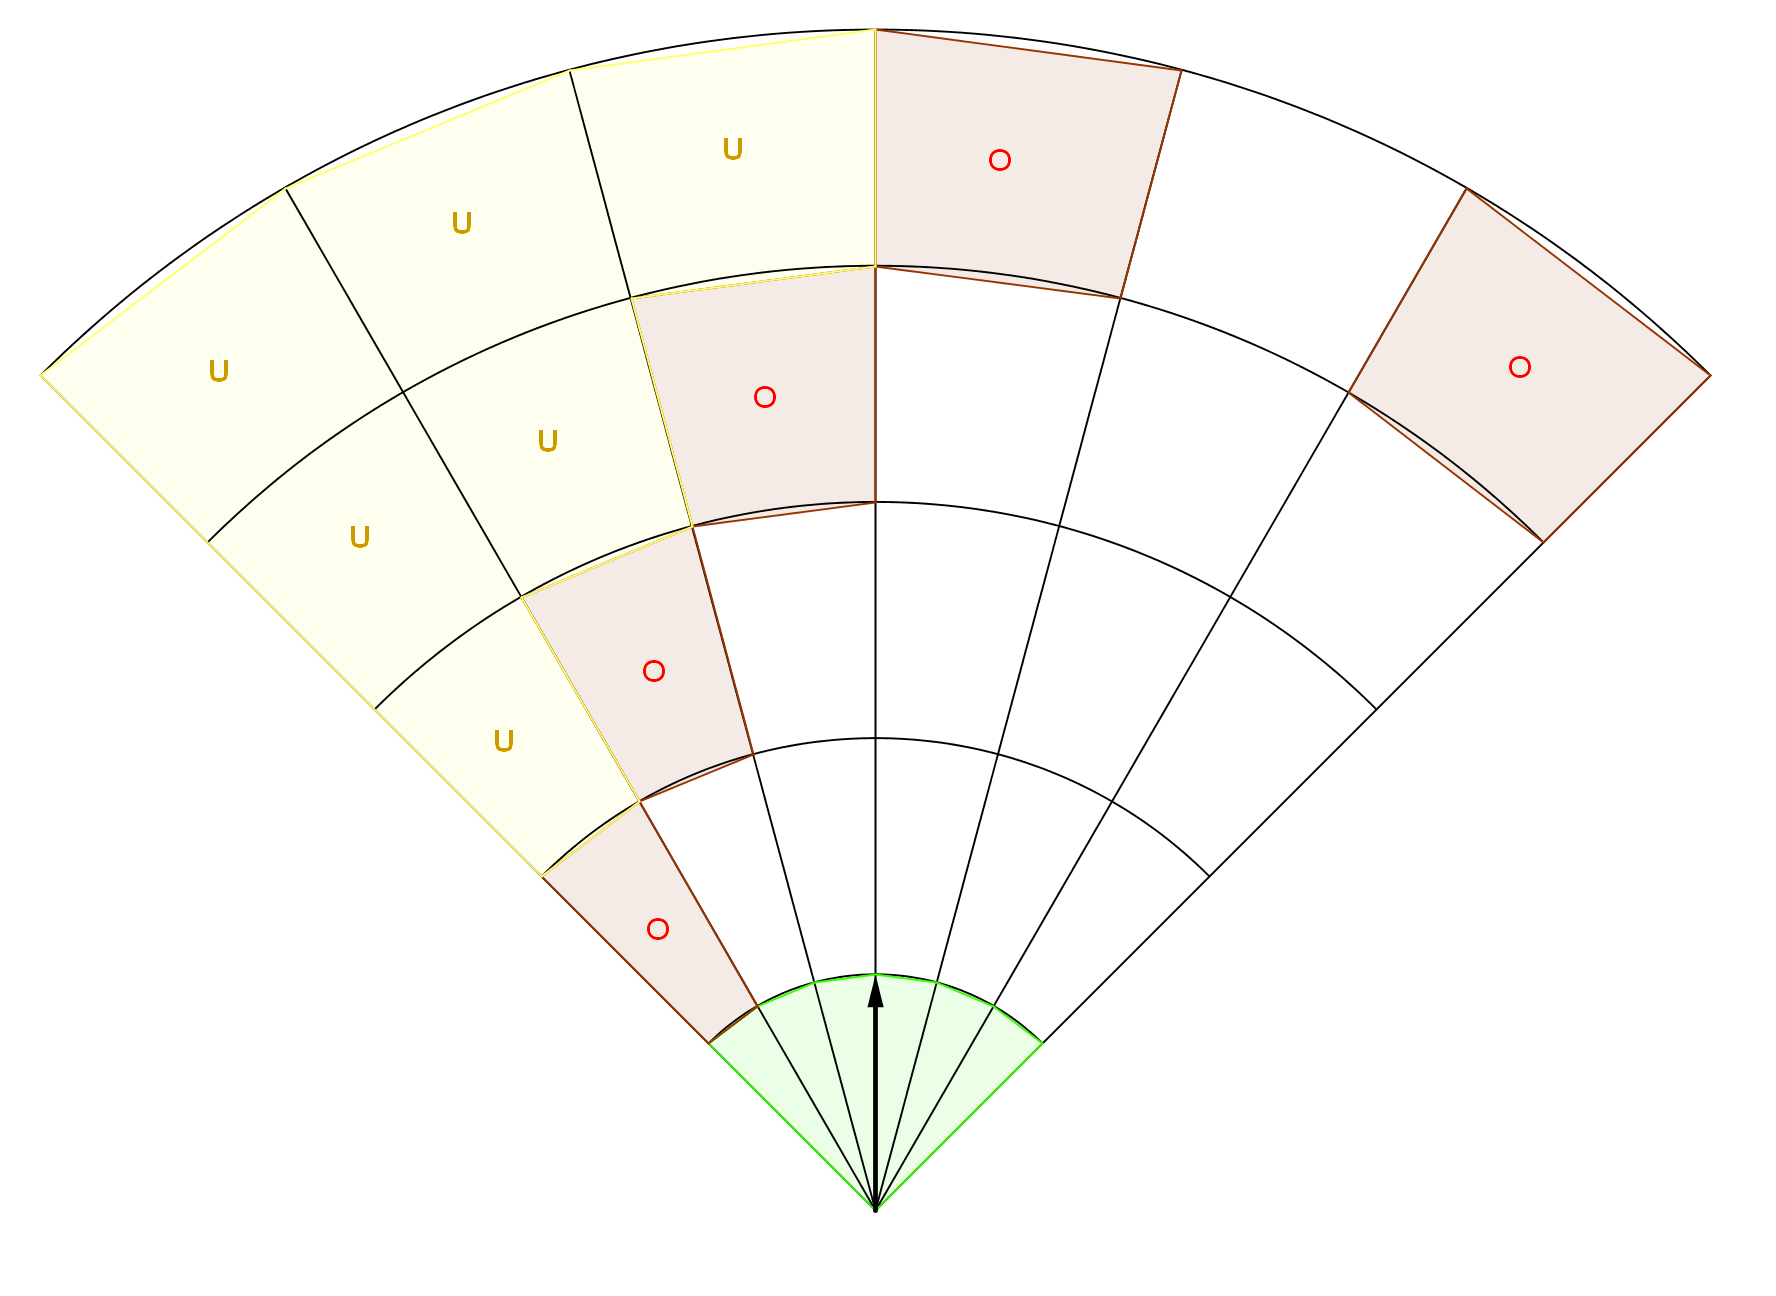
\includegraphics[width=0.9\linewidth]{\FIGDIR/CA002UncertainityAssesment} 
        \caption{Uncertainty assessment.}
        \label{fig:uncertainityAssesmentAvoidanceGrid}
    \end{subfigure}
    \\
    \begin{subfigure}{0.48\textwidth}
        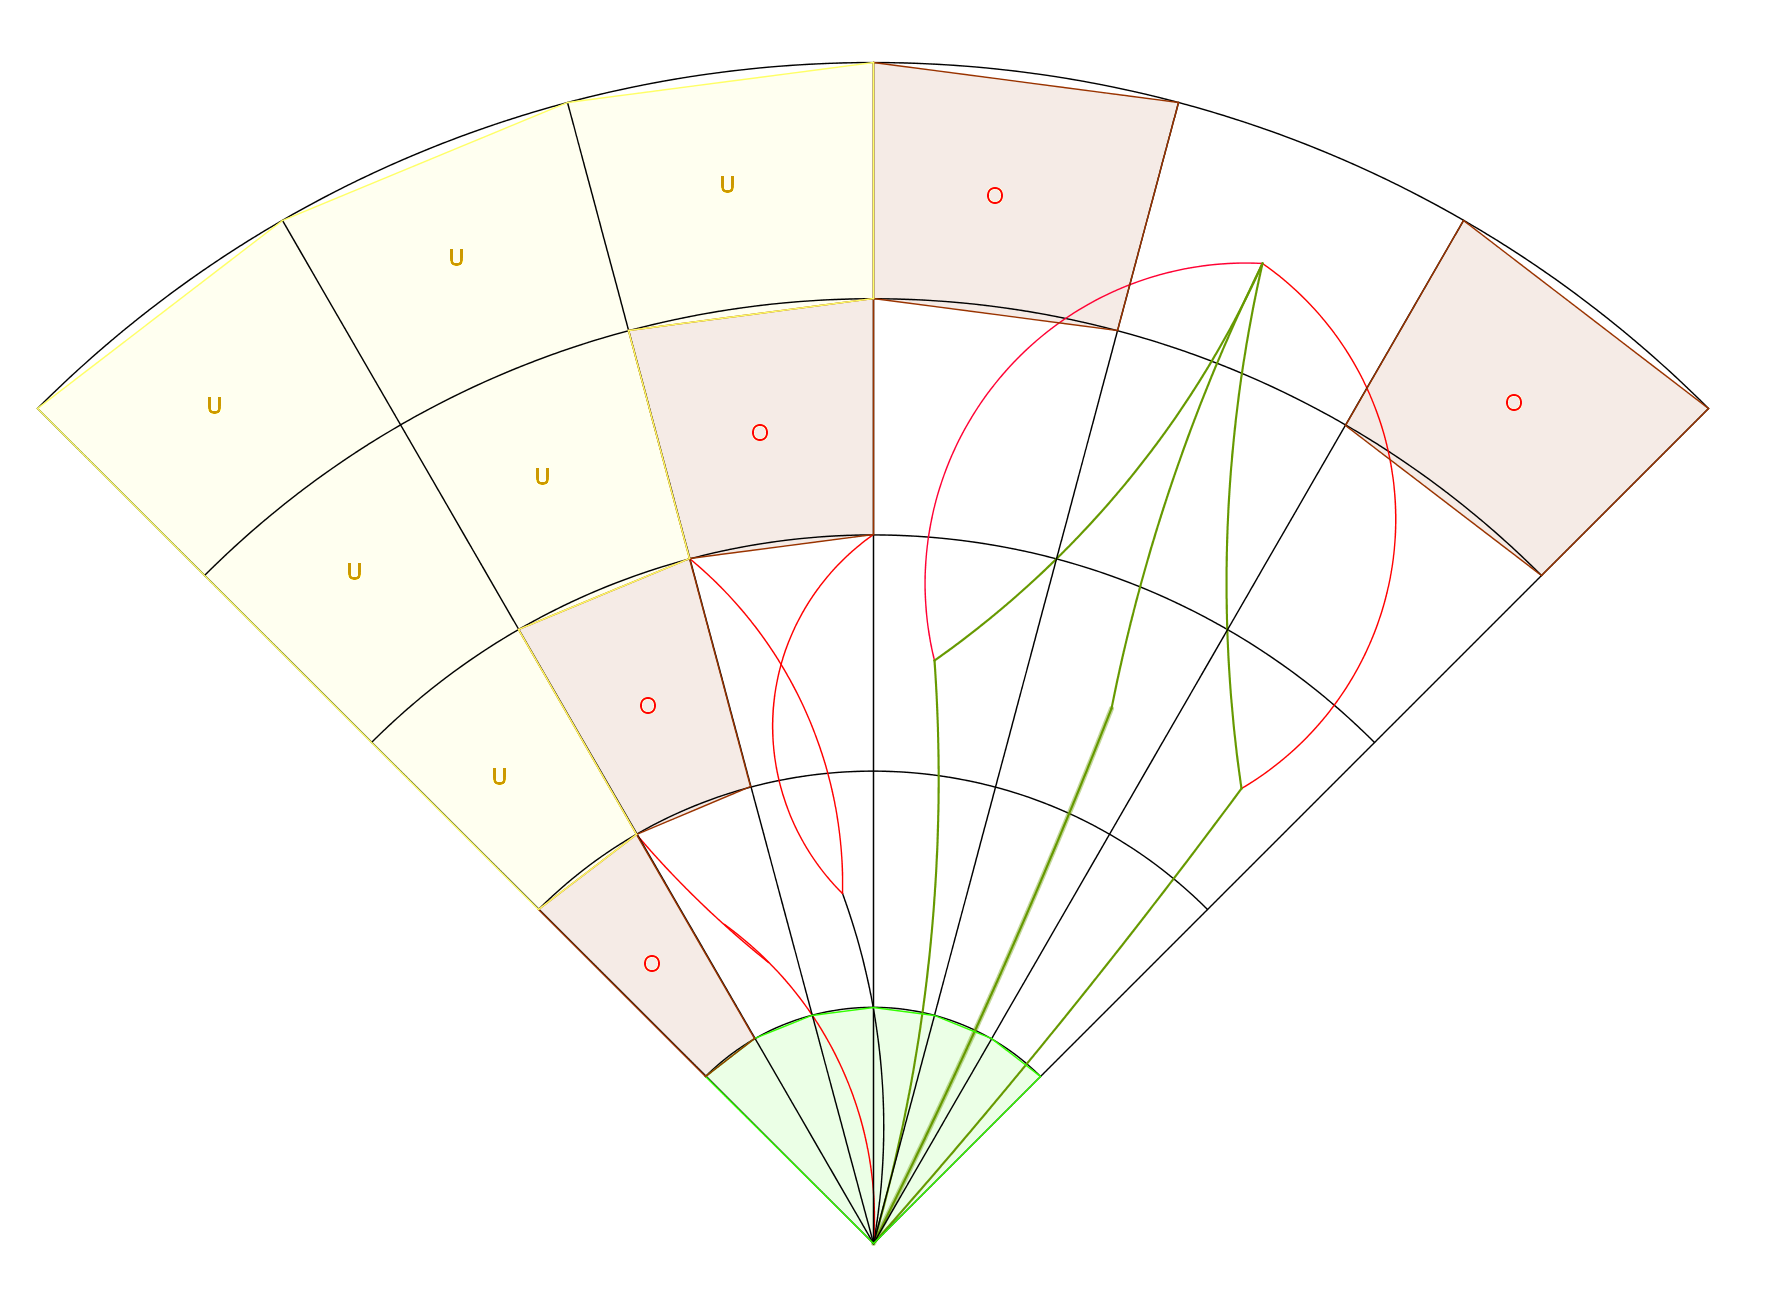
\includegraphics[width=0.9\linewidth]{\FIGDIR/CA003SurveyOfVacantSpace} 
        \caption{Trajectories reachibility evaluation.}
        \label{fig:trajectoriesSafetyEvaluationAvoidanceGrid}
    \end{subfigure}
    \begin{subfigure}{0.48\textwidth}
        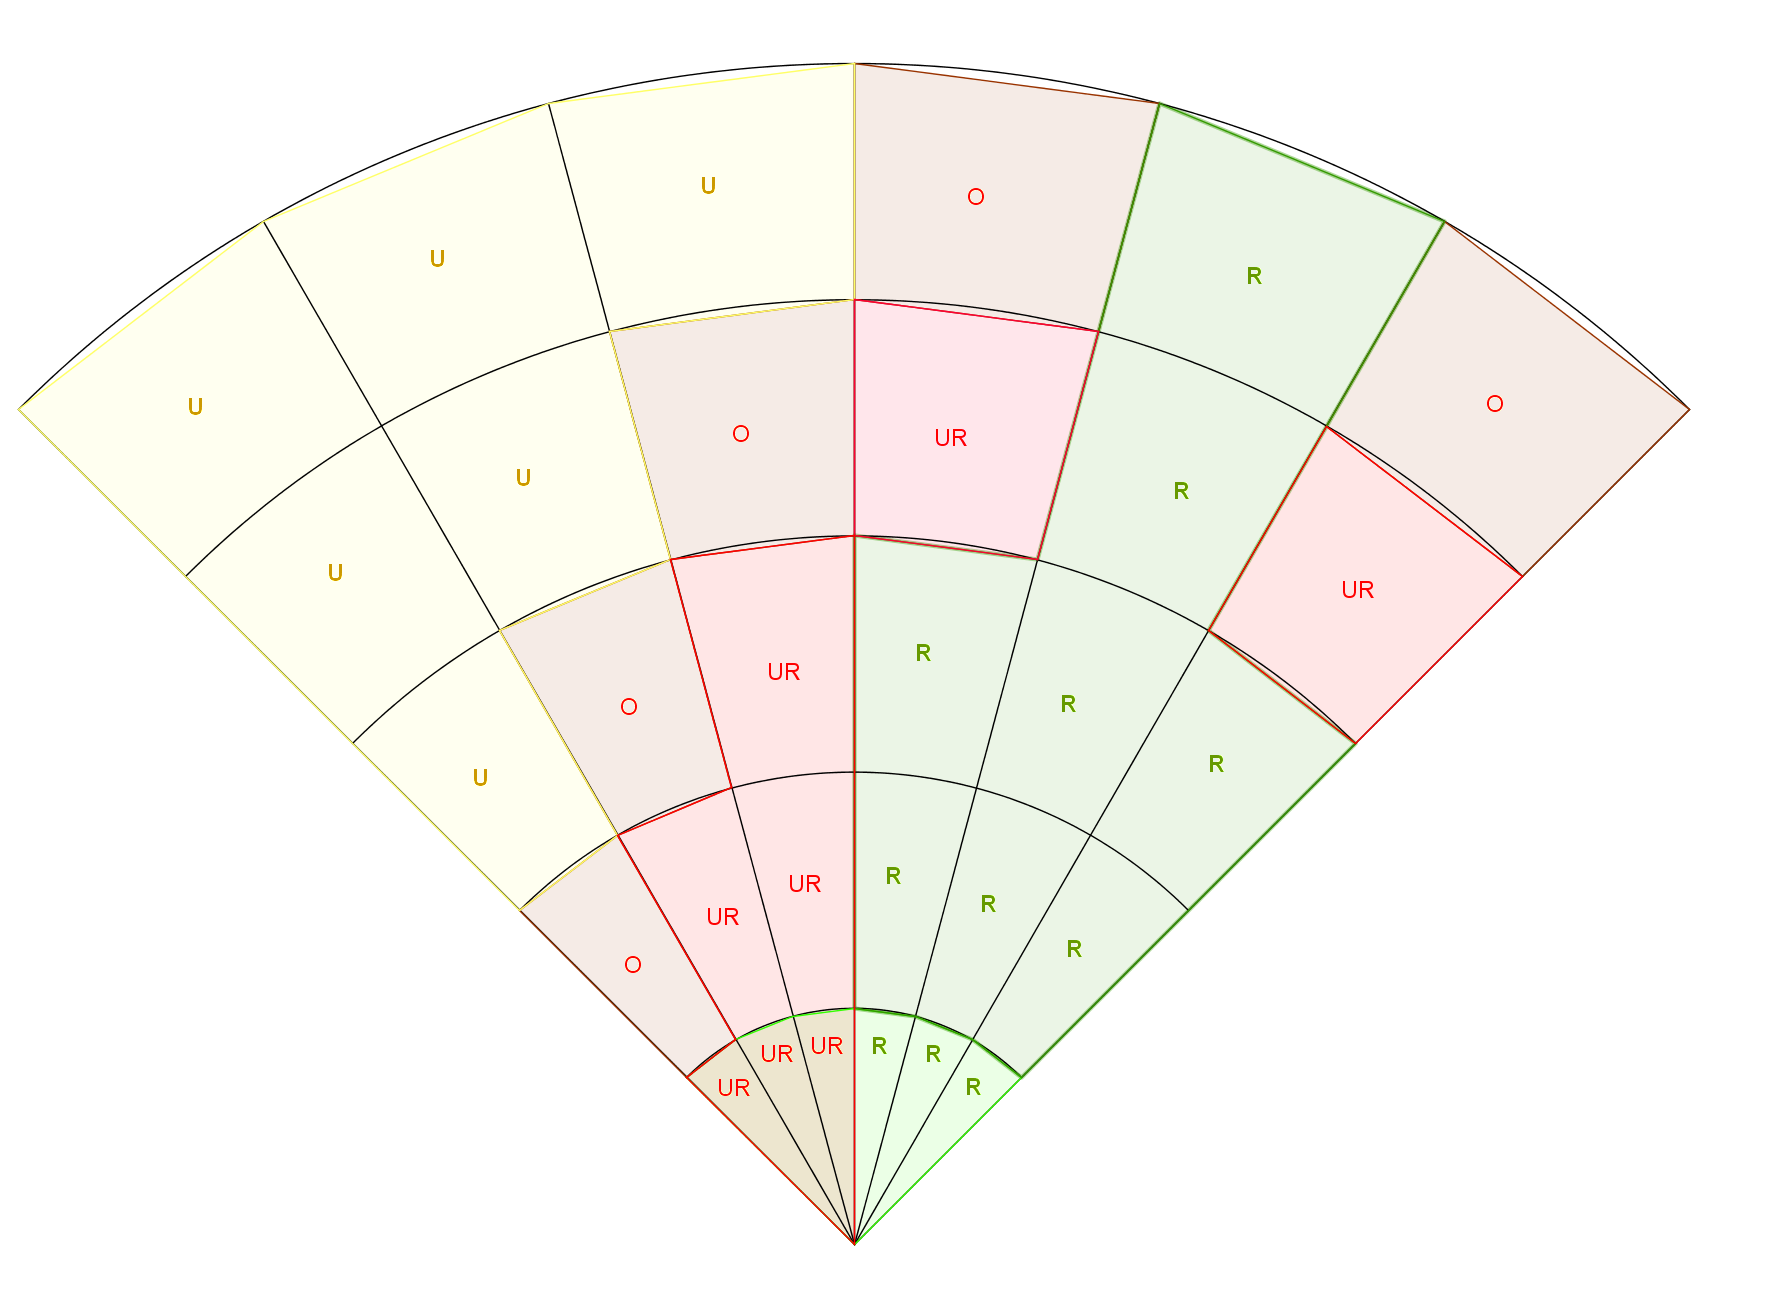
\includegraphics[width=0.9\linewidth]{\FIGDIR/CA004ReachableSpaceAssesment} 
        \caption{Cell reachibility evaluation.}
        \label{fig:reachibilityAssessmentAvoidanceGrid}
    \end{subfigure}
    \caption{Significant steps of \emph{Avoidance grid run} (inner loop).}
    \label{fig:significantStepsofAvoidanceGridRun}
\end{figure}

\begin{note}
    The \emph{Sensor Fusion Procedure} is solving all following steps (sec. \ref{s:sensorFusion}). The \emph{main purpose} of \emph{Avoidance Run} is finding best path under certain conditions.
\end{note}

\paragraph{Space Assessment Principle:} The \emph{Avoidance Grid} is fed trough \emph{Data Fusion} (sec. \ref{s:sensorFusion}). The process of \emph{ratings assessment} (tab. \ref{tab:defuzificationRatings}) is given in (fig. \ref{fig:significantStepsofAvoidanceGridRun}):
\begin{enumerate}
    \item \emph{Obstacle detection} (fig. \ref{fig:obstacleDetectionAvoidanceGrid}) - assessment of \emph{detected obstacles} (eq. \ref{eq:detectedObstacleRatingForCell}). The red (O) $cells$ have Detected obstacle set as \emph{true}. The other threats: \emph{map obstacles} (eq. \ref{eq:mapObstacleRatingForCell}), \emph{intruders} (eq. \ref{eq:intruderRatingForCell}), \emph{constraints} (eq. \ref{eq:constraintRatingForCell}) are false. The red (0) $cells$ are representing $Occupied(t_i)$ (eq. \ref{eq:ocuupiedDataFusion}) space in \emph{Avoidance Grid} at decision time $t_i$.
    
    \item \emph{Uncertainty assessment} (fig. \ref{fig:uncertainityAssesmentAvoidanceGrid}) - the uncertain cells are cells which status can not be \emph{assessed}. The \emph{Visibility} (eq. \ref{eq:visibilityForCell}) is low. The \emph{Uncertain} cells (yellow (U) mark) are equal to $Uncertain(t_i)$ (eq. \ref{eq:UncertainDataFusion}) in \emph{Avoidance Grid} in \emph{decision time} $t_i$. The $Constrained(t_i)$ (eq. \ref{eq:ocuupiedDataFusion}) space is equal to $\varnothing$ in this example.
    
    \item \emph{Trajectory reachibility evaluation} (fig. \ref{fig:trajectoriesSafetyEvaluationAvoidanceGrid}) - the \emph{Reach Set} given as \emph{Trajectory Set} (eq. \ref{eq:trajectoryTree}). is then projected trough \emph{Avoidance Grid} and pruned according to (def. \ref{def:PrunedReachSet}). \emph{Reachable Trajectories} (eq. \ref{eq:trajectoryReachibility}) are only those contained in $Free(t_i)$ space (eq. \ref{eq:freeDataFusion}). The \emph{Reachable Trajectories} are denoted as \emph{green lines}. The \emph{Unreachable} trajectory segments are denoted as \emph{red lines}. 
    
    \item \emph{Cell reachibility evaluation} (fig. \ref{fig:reachibilityAssessmentAvoidanceGrid}) - the evaluation of $cells$ reachibility is going according to (eq. \ref{eq:cellReachibility}). The \emph{Reachable cells} are those which \emph{contains} at least one \emph{Reachable Trajectory Segment}.
\end{enumerate}



\paragraph{Finding Best Path:} \footnote{Avoidance Run Function Implementation:\url{RuleEngine/MissionControl/MissionControl.m::findBestPath(avoidanceGrid)}} Each $cell_{i,j,k}$ in \emph{Avoidance Grid} at \emph{decision time} $t_i$ has assessed ratings according to \emph{data fusion procedure} (tab. \ref{tab:defuzificationRatings}). The following properties are know prior the \emph{trajectory} selection:
\begin{enumerate}
    \item \emph{Reachibility} for each  $cell_{i,j,k}$ (eq. \ref{eq:cellReachibility}).
    \item \emph{Reachibility} for each  $Trajectory(\circ)$ (eq. \ref{eq:trajectoryReachibility}).
    \item \emph{Free Space} as non empty set of $cells$ in \emph{Avoidance Grid} (eq. \ref{eq:freeDataFusion}), with \emph{Reachable Space} (eq. \ref{eq:ReachableDataFusion}).
    \item \emph{Goal Waypoint} $\mathscr{WP}_G$ from \emph{Mission Control Run} (sec. \ref{s:missionControlRun}).
\end{enumerate}

The \emph{Algorithm} (alg. \ref{alg:FindBestPathAvoidanceGrid}) is based on \emph{shortest path} search. Navigation is trying to reach \emph{goal waypoint}, therefore it tries to shorter distance between \emph{trajectory final cell} and \emph{goal waypoint}. If there is \emph{reachable space} two situations can occur:
\begin{enumerate}
    \item \emph{Goal waypoint is inside the Avoidance Grid} - the \emph{avoidance cell} is cell$_{i,j,k}$ containing \emph{goal waypoint} if reachable. 
    
    \item \emph{Goal waypoint is outside the Avoidance Grid} - the \emph{avoidance cell} is closest cell considered as \emph{outer cell} to \emph{goal waypoint}.
\end{enumerate}

\begin{note}
    \emph{Outer cell} is a cell$_{i,j,k}$ which has at least one \emph{wall} directly neighbouring with \emph{outer space} ($Universe - Known World (t_i)$). The \emph{outer cell} is selected to prevent navigation to the \emph{trap}.
\end{note}

The \emph{Avoidance Path} selection is simple lowest cost selection of \emph{Trajectory} $\in$ cell$_{i,j,k}$.
\newpage

\begin{algorithm}[H]
\SetKwInOut{Input}{Input}
\SetKwInOut{Output}{Output}
\Input{Cell[]  reachable (eq. \ref{eq:ReachableDataFusion}), Waypoint goal, AvoidanceGrid($t_i$) grid}
    
\Output{Trajectory avoidancePath, Error message}
    
    \BlankLine
    \# Initialization \& Reachibility test\;    
    avoidancePath = $\varnothing$\;
    \If{reachable ==  $\varnothing$}{        
        message = "No path available, empty Reach Set"\;
        \Return{[avoidancePath,message]}
    }
    avoidanceCell = GetRandomCell(reachable)\;
    
    \BlankLine
    \# Look for for goal cell\;
    \eIf{goal $\in$ grid}{
        \BlankLine
        \# Goal is inside Avoidance Grid, Check if reachable\;
        avoidanceCell = grid.selectCellXYZ(goal)\;
        \If{avoidanceCell.Reachable != true}{
            message = "Waypoint not Reachable"\;
            \Return{[avoidancePath,message]}
        }
    }{
        \BlankLine
        \# Goal is outside Avoidance Grid, look for closest reachable cell$_{i,j,k}$\;
        minimalDistance = distance(avoidanceCell,goal)\;
        \For{cell$_{i,j,k}$ $\in$ reachable}{
            
            \If{distance(cell$_{i,j,k}$,goal) $<$ minimalDistance}{
                \If{isOuterCell(cell$_{i,j,k}$)}{
                    minimalDistance = distance(cell$_{i,j,k}$,goal)\;
                    avoidanceCell = cell$_{i,j,k}$\;
                }
            }
        }
    }
    
    \BlankLine
    \# Reachable cell was found, Look for cheapest reachable trajectory\;
    avoidancePath = GetRandomTrajectory(avoidanceCell)\;
    \For{trajectory $\in$ avoidance Cell \&\& trajectory.Reachable == true}{
        \If{trajectory.Cost $<$ avoidancePath.cost}{
            avoidancePath = trajectory\;
        }
    }
   
    message = $\varnothing$\;
    \Return{[avoidancePath,message]}
    
    \caption{Find best \emph{Path} in \emph{Avoidance Grid}}
    \label{alg:FindBestPathAvoidanceGrid}    
\end{algorithm}

\newpage
\paragraph{Space Assessment Example:} For better understanding there is following example of \emph{space assessment} and \emph{Best Path Selection}. 


The \emph{UAS} (blue plane) is following \emph{mission plan} in open space. Then there is a detection of an \emph{collision situation} (fig. \ref{fig:exampleSituationAvoidanceRun}). The \emph{Obstacle} is detected in \emph{top-right} Avoidance Grid corner. 

The \emph{LiDAR hits} are denoted as red filled circles. The \emph{Avoidance Grid} space is constrained by black dashed line. The \emph{Avoidance Grid} is separated into 5 layers going from top to \emph{bottom}. The \emph{Reach Set} is projected as a set of \emph{Trajectories} with colorization. 

\begin{figure}[H]
\centering
    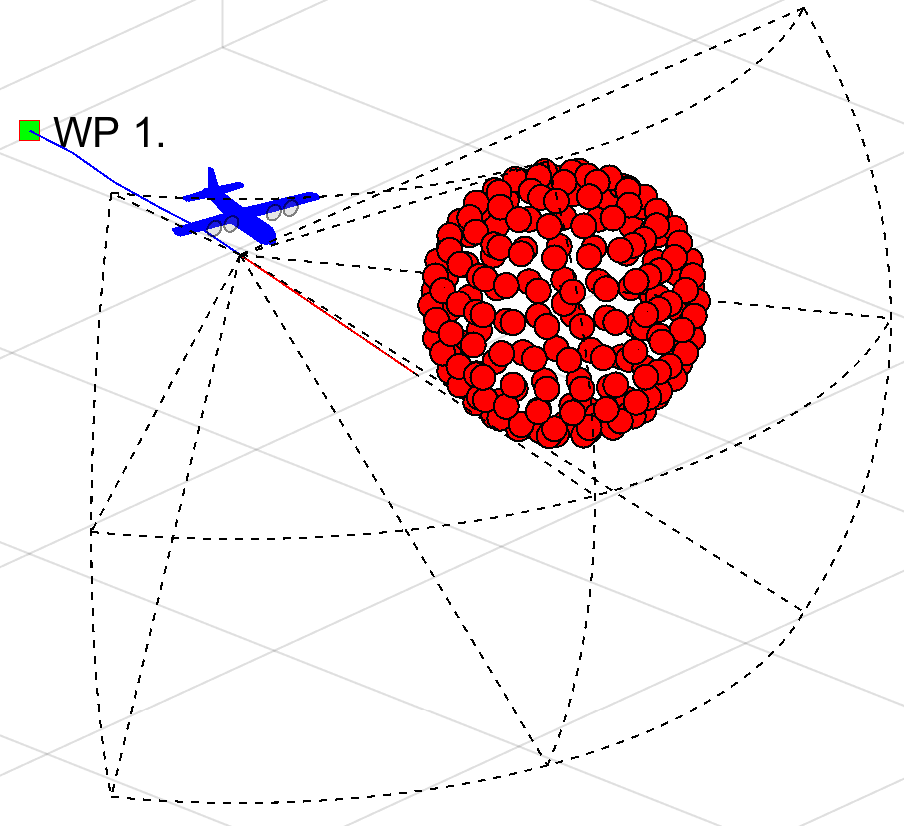
\includegraphics[width=0.75\linewidth]{\FIGDIR/TE038AvoidanceRunExample}        
    \caption{Example: The situation to be evaluated by \emph{Avoidance Run}.}
    \label{fig:exampleSituationAvoidanceRun}
\end{figure}
\newpage
\noindent\emph{Visibility Assessment:} The visibility assessment (fig. \ref{fig:exampleVisibilityEvaluation}) divides the \emph{Avoidance Grid} into two
\begin{enumerate}
    \item \emph{Visible space} (blue filled cells) is space \emph{trough} which \emph{LiDAR} rays roamed freely until they hit an \emph{Obstacle}.
    
    \item \emph{Uncertain space} (black filled cells) is space where no \emph{LiDAR ray} passed nor hit. Therefore its status is uncertain.
\end{enumerate}
 
 \begin{note}
     The \emph{detected obstacle cells} are part of \emph{visible space}, because there is certainty about its containment.
 \end{note}
 
 The \emph{Reach Set} trajectories are colored based on their visibility, blue for \emph{uncertain} trajectories and \emph{green} for visible trajectories.

\begin{figure}[H]
    \centering
    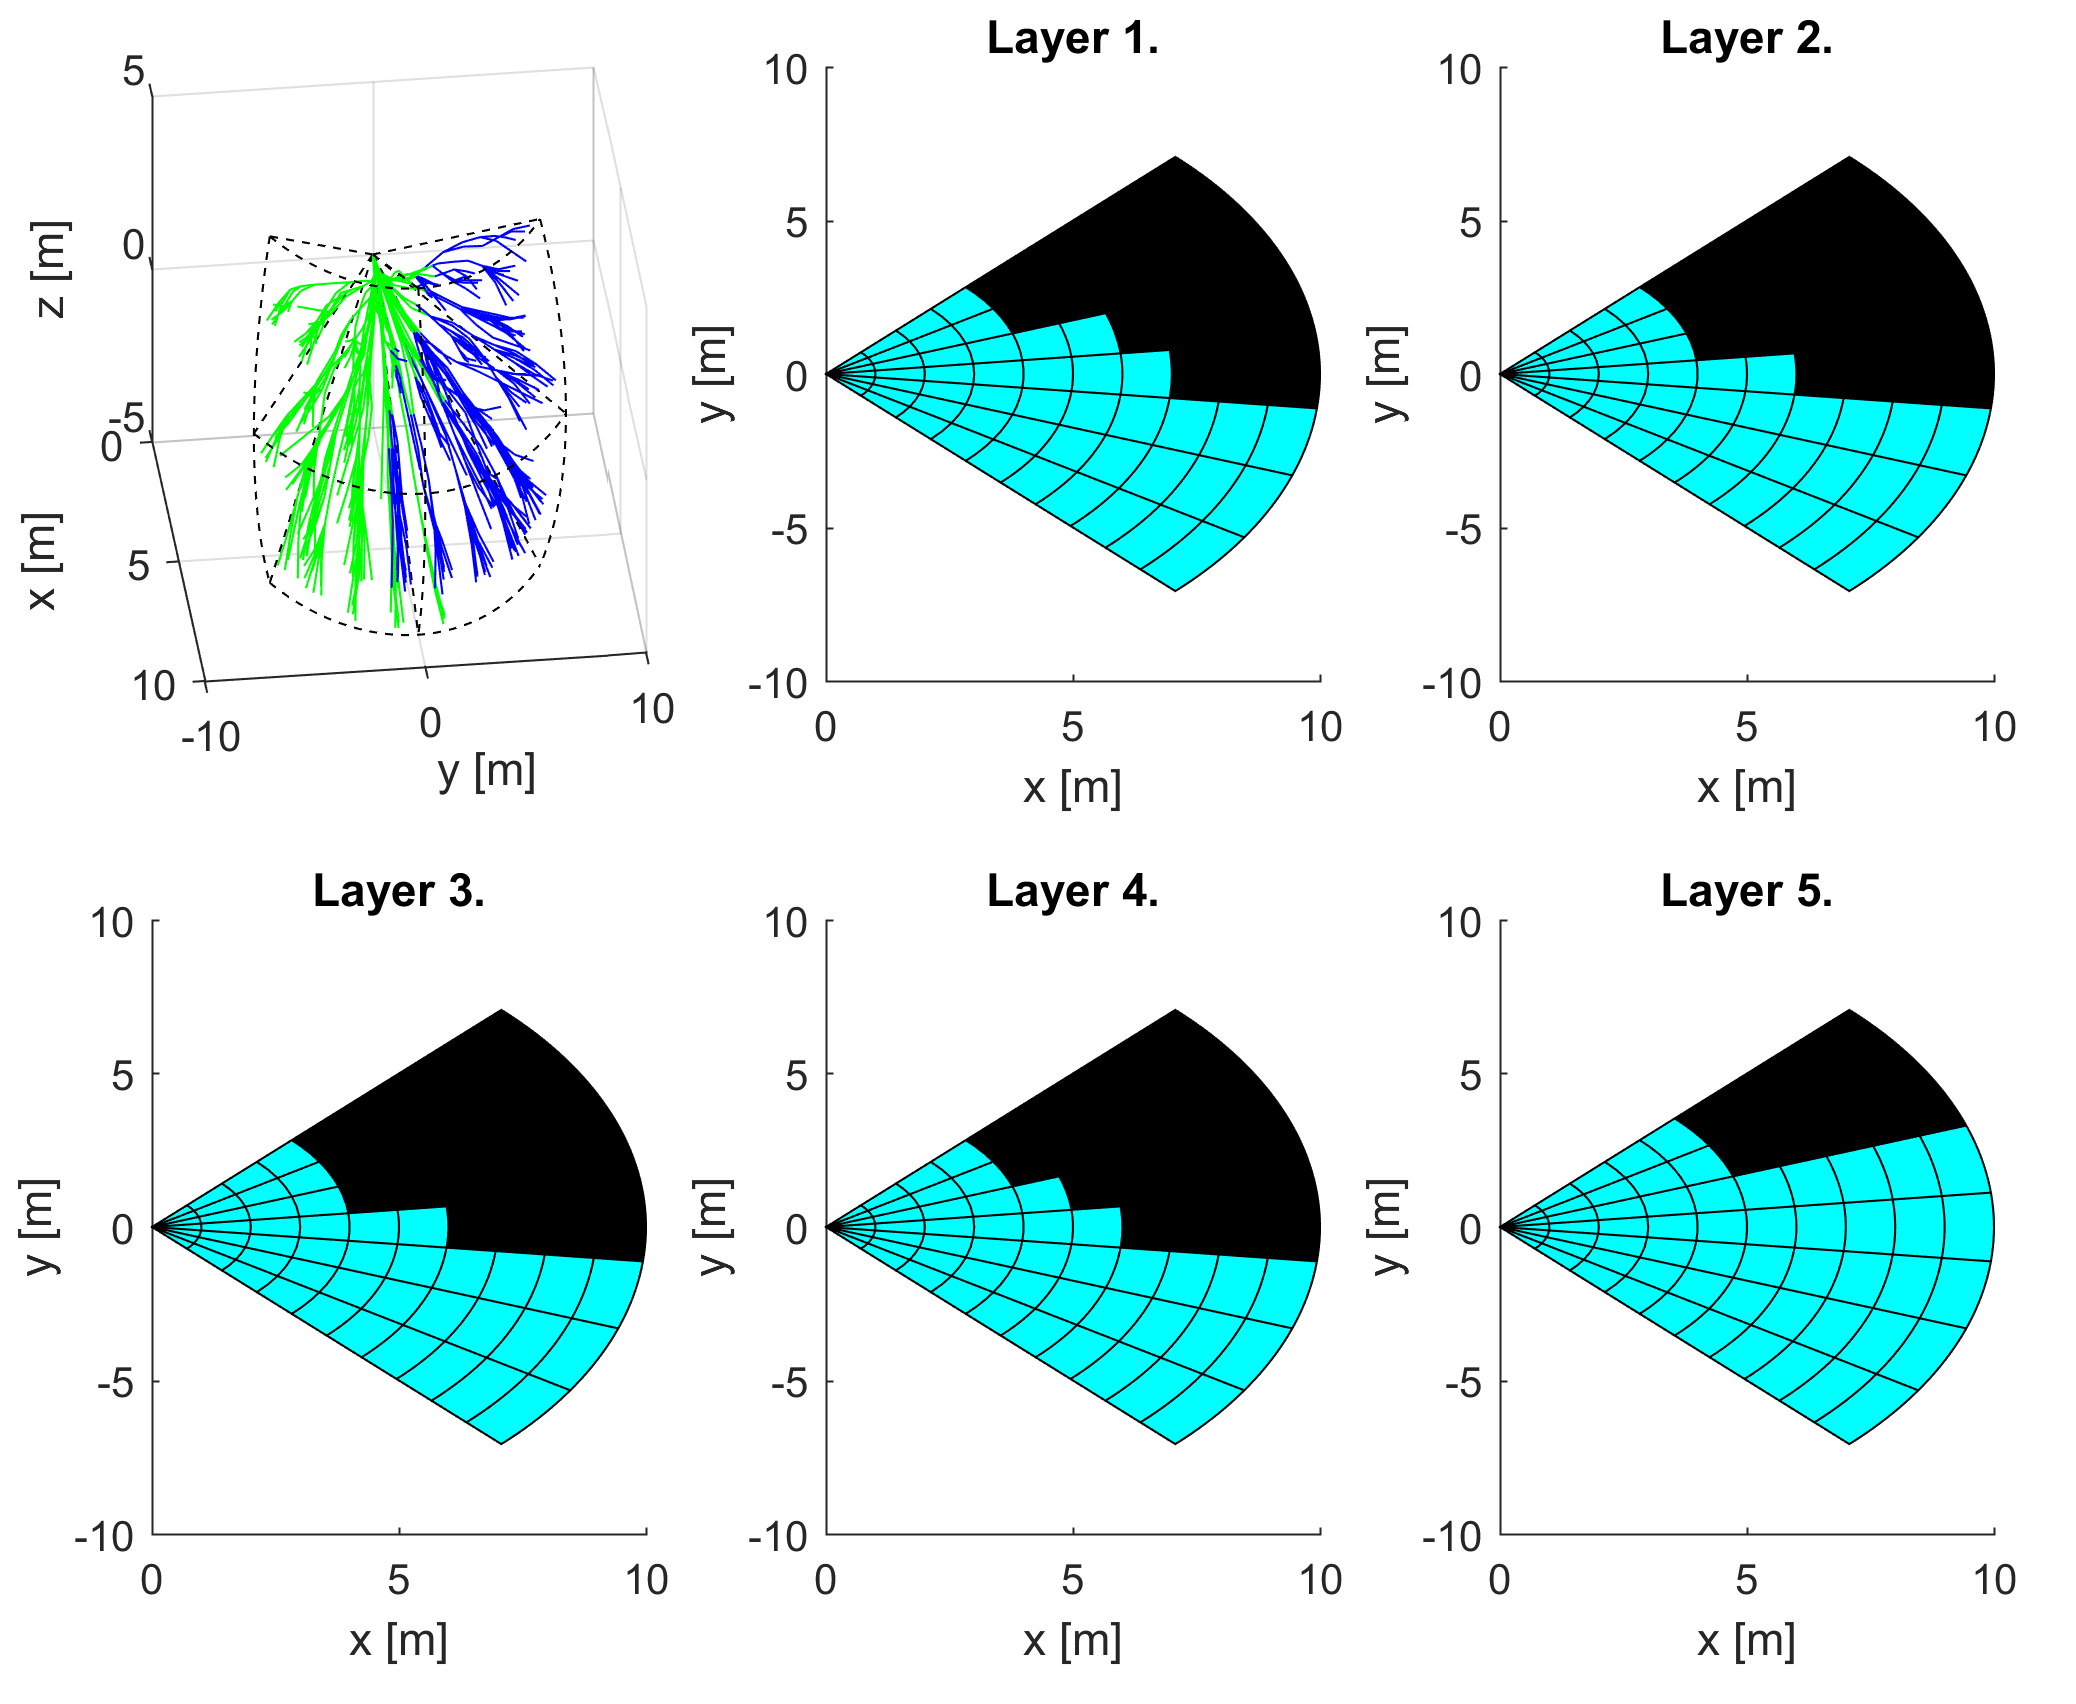
\includegraphics[width=0.95\linewidth]{\FIGDIR/TE040Visibility}        
    \caption{Example: The \emph{Visibility} evaluation by \emph{Avoidance Run}.}
    \label{fig:exampleVisibilityEvaluation}
\end{figure}

\newpage
\noindent\emph{Reachibility Assessment:} For Each trajectory the \emph{Reachibility} is assessed (fig. \ref{fig:exampleReachibilityEvaluation}). The \emph{Obstacle Space} and \emph{Uncertain Space} are rendering \emph{reachibility}, effectively separating \emph{trajectories} into two categories:

\begin{enumerate}
    \item \emph{Unreachable Trajectories} (red lines) - there is at least one trajectory segment leading trough \emph{Obstacle} or \emph{Uncertain} space.
    
    \item \emph{Reachable Trajectories} (green lines) -  all trajectory segments are lying in \emph{Free} space.
\end{enumerate}

Cells in Avoidance grid are divided in similar matter, depending on count of \emph{reachable trajectories} passing trough them:

\begin{enumerate}
    \item \emph{Unreachable Cells} (red fill) - there is no trajectory trough \emph{free space} or the \emph{cell} is not in \emph{free space}.
    
    \item \emph{Reachable cells} (green fill) - there is at least one \emph{feasible trajectory} reaching \emph{free cell}.
\end{enumerate}

\begin{figure}[H]
    \centering
    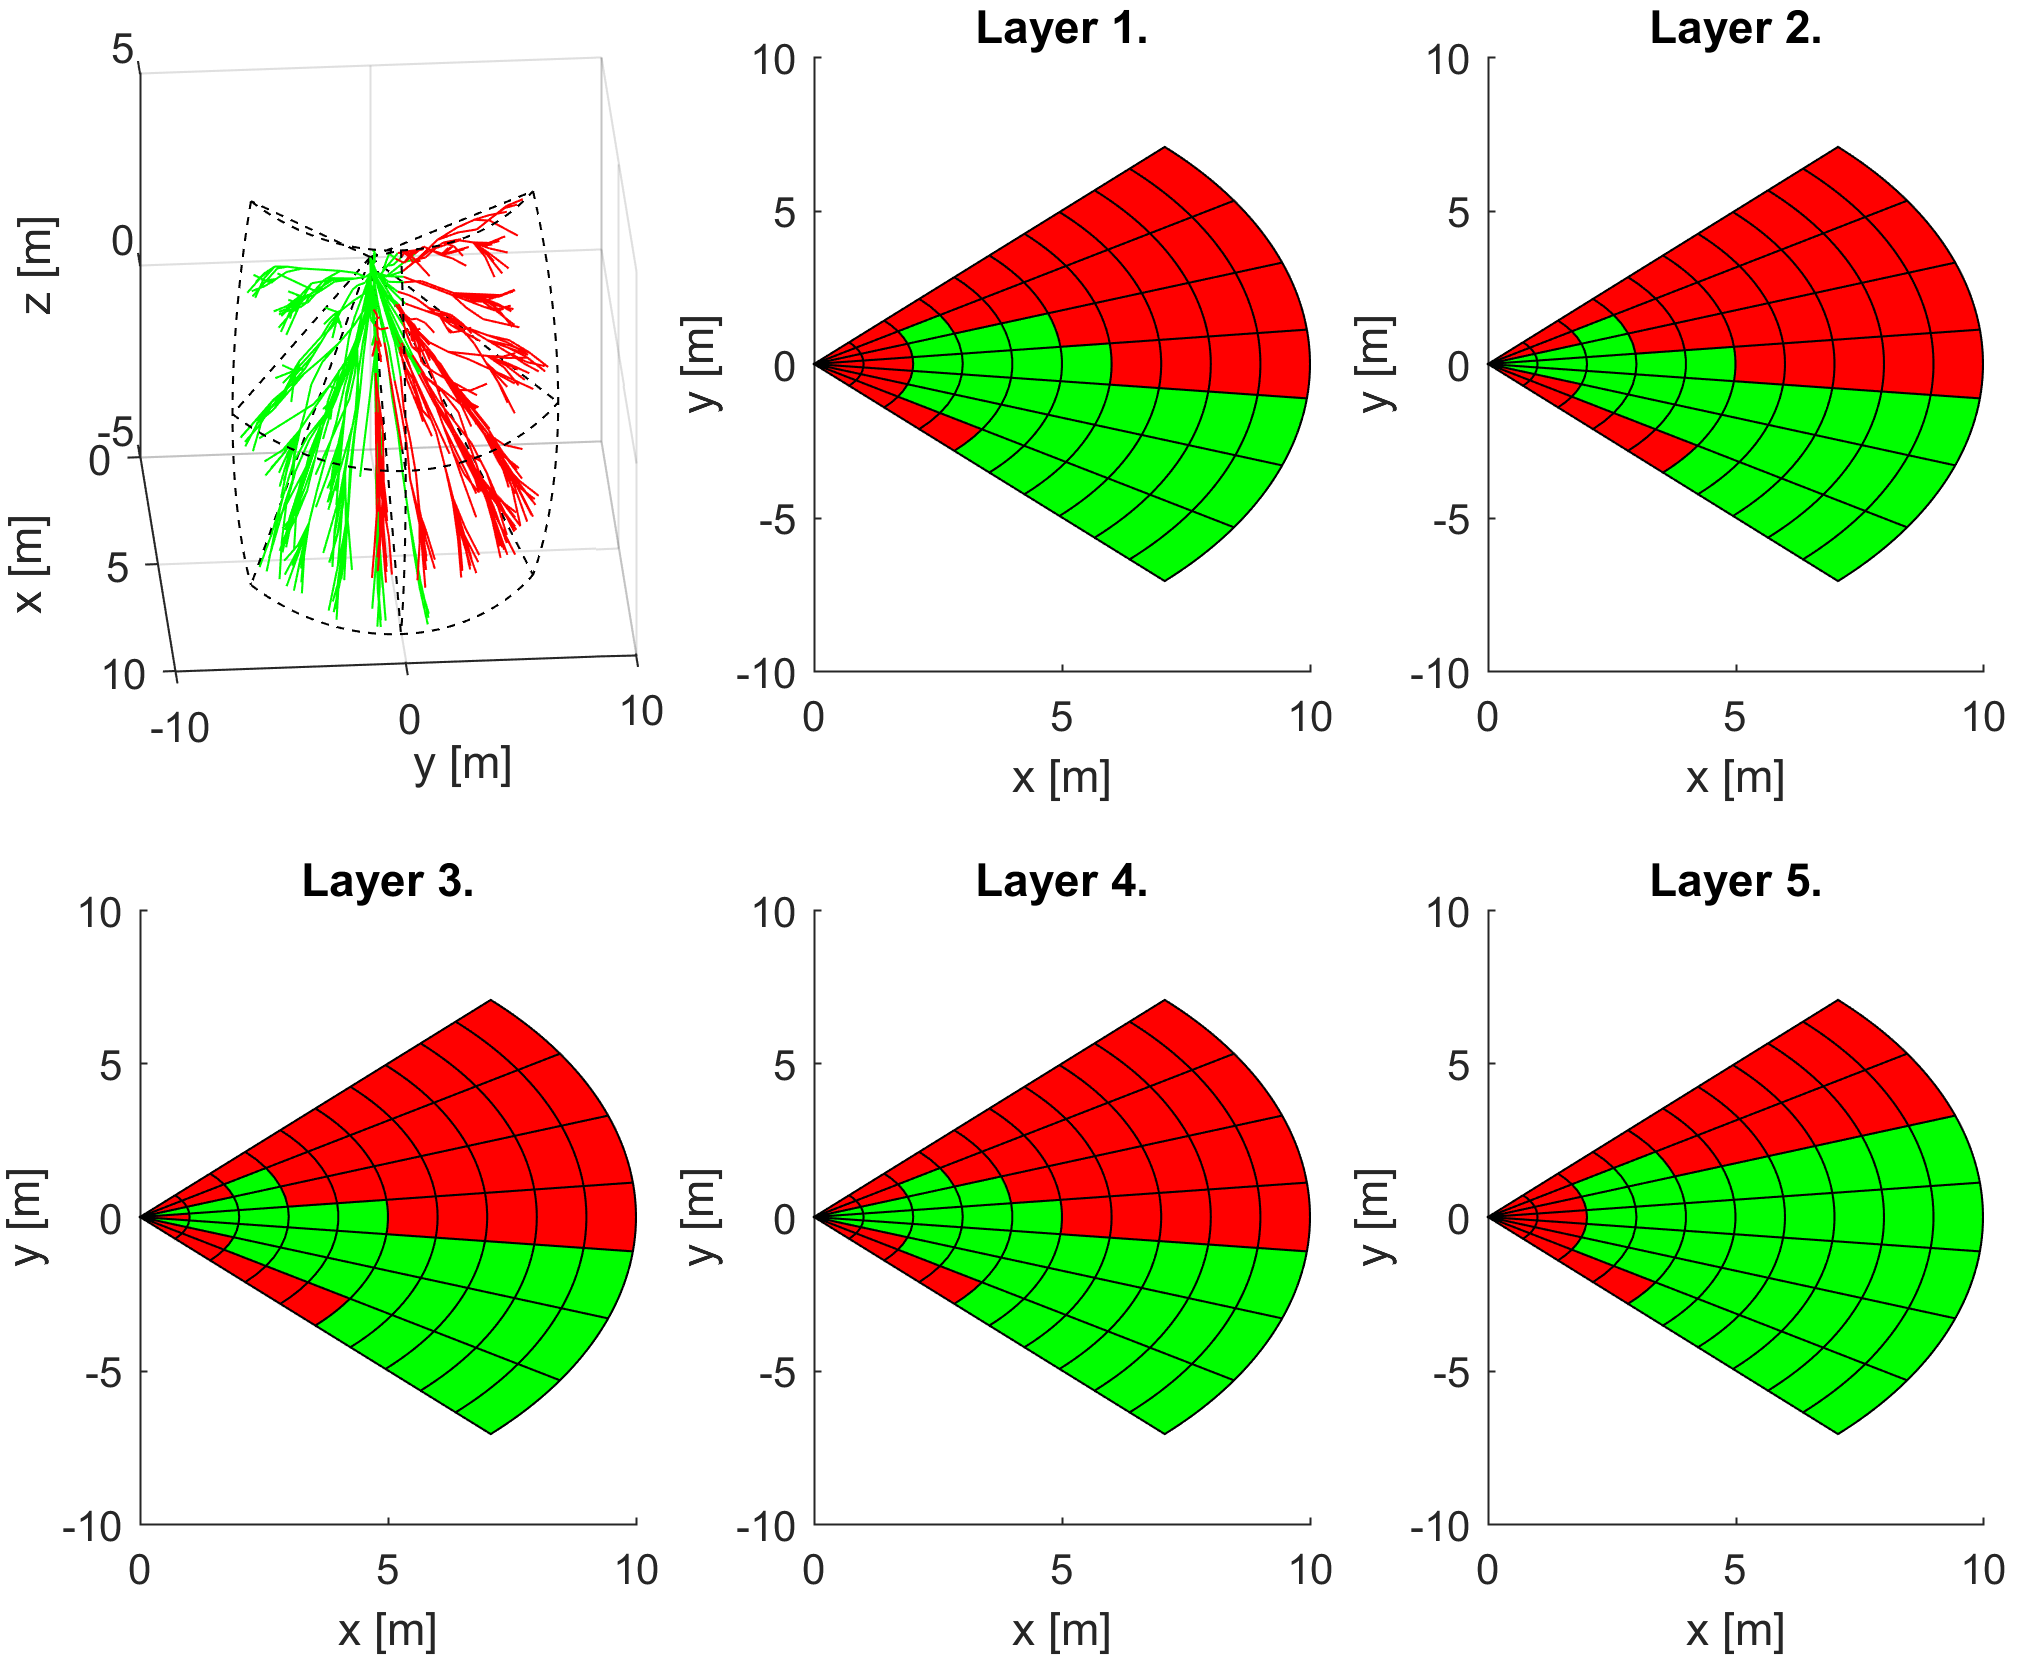
\includegraphics[width=0.95\linewidth]{\FIGDIR/TE041Reachibility}        
    \caption{Example: The \emph{Reachibility} evaluation by \emph{Avoidance Run}.}
    \label{fig:exampleReachibilityEvaluation}
\end{figure}

\begin{note}
    The \emph{best avoidance path} is selected form \emph{reachable outer cells} (green fill in fig. \ref{fig:exampleReachibilityEvaluation}), depending on \emph{goal waypoint} according to (alg. \ref{alg:FindBestPathAvoidanceGrid}).
\end{note}
    	\newpage
\subsection{\secState{R}Mission Control Run}\label{s:missionControlRun}
\paragraph{Introduction and Motivation:}  This section will introduce \emph{Navigation Concept} using  \emph{Reach Set Approximation}. The \emph{Avoidance Framework Concept} (fig. \ref{fig:AvoidanceFrameworkConceptNew}) defines \emph{Navigation Module} as \emph{sub-system} for long term \emph{trajectory tracking}.  The \emph{Avoidance Grid Run} (sec. \ref{s:aviudabceGridRun}) is solving the \emph{Path Search} problem inside operation space constrained by \emph{Avoidance Grid} for time $t_i$. 

There is a need to build a trajectory between \emph{Waypoints} which are further away than \emph{distance} of one \emph{Avoidance Grid}.  The \emph{UAS} is controlled via \emph{Movement Automaton}. The \emph{Movements} which are in \emph{Movement Buffer} can be replaced with another movements. This feature of \emph{Movement Automaton} is called \emph{Movement Chaining} (eq. \ref{eq:movementChaining}).

To join the multiple \emph{Avoidance Grids} paths following terminology needs to be established (fig. \ref{fig:missionControlRunExample}):
\begin{enumerate}
    \item \emph{Goal} (Selecting Goal of Navigation) - the point where UAS want to get in global coordinate frame. The selection needs to be defined.
    
    \item \emph{Next Decision} - the point when the next \emph{Avoidance Grid Run} is applied. The outline of events and triggers is required. The \emph{decision} will be made in \emph{next decision time} $t_{i+1}$.
\end{enumerate}

\noindent The \emph{Avoidance Grid} from \emph{UAS} viewpoint can be separated into following zones (fig. \ref{fig:gridZonesMissionControl}):
\begin{enumerate}
    \item \emph{Crash Area} (last layers) - there is no place for safe return and the \emph{border} of \emph{Avoidance Grid} is near. The \emph{Decision Point} needs to lie before this zone.
    
    \item \emph{Avoidance Area} (middle layers) - the area of \emph{Active Avoidance Maneuvering}. The \emph{Reach Set Approximation} performance (sec. \ref{s:ReachSetPerformanceCriteria}) is important in this area.
    
    \item \emph{Safe Zone} (first layers) - there is space for safe return or damage mitigation.
\end{enumerate}

\begin{figure}[H]
    \centering
    \begin{subfigure}{0.48\textwidth}
        \centering
        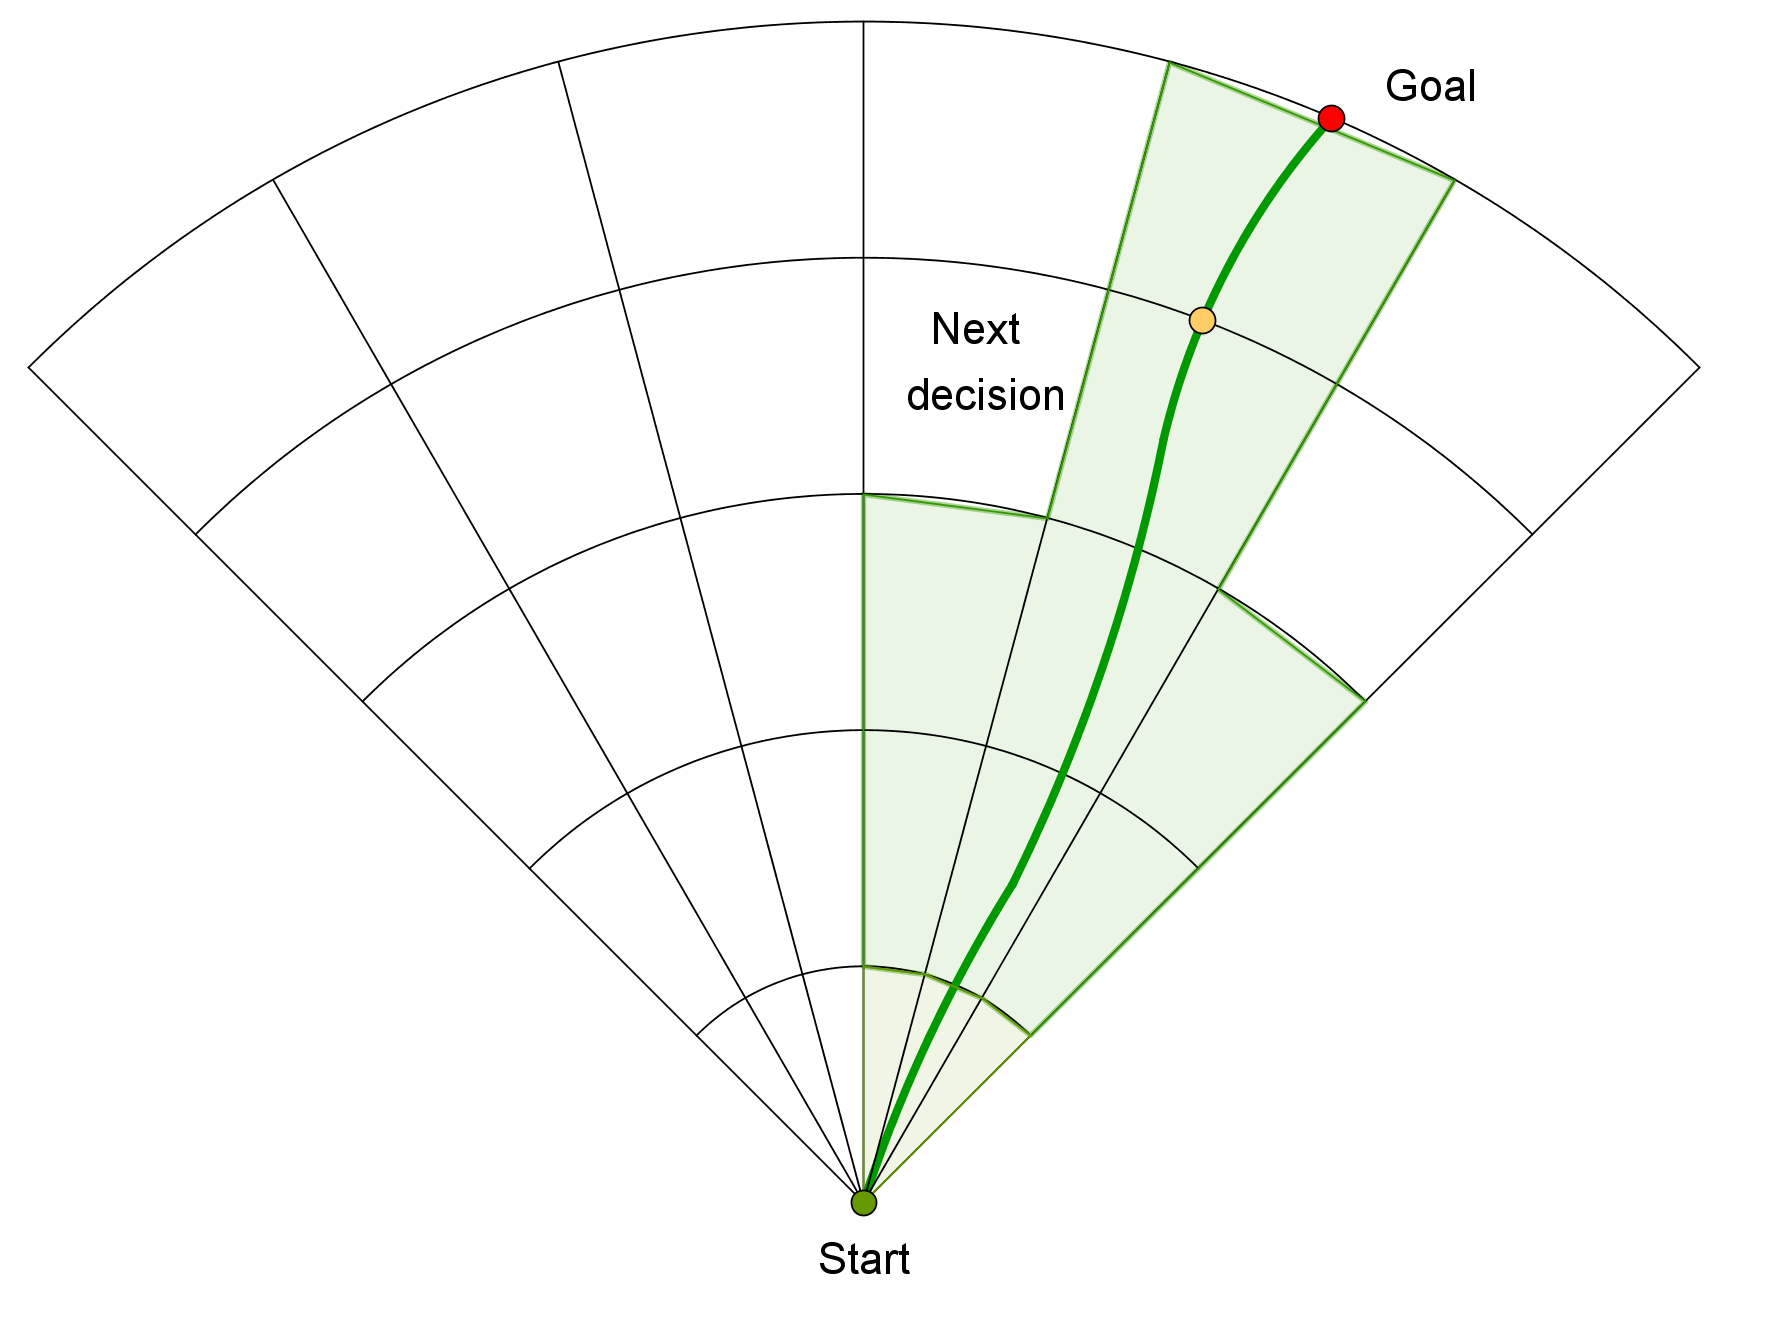
\includegraphics[width=0.9\linewidth]{\FIGDIR/CA005PathCalculation}
        \caption{Mission control run example.}
        \label{fig:missionControlRunExample}
    \end{subfigure}
    \begin{subfigure}{0.48\textwidth}
    	\centering
        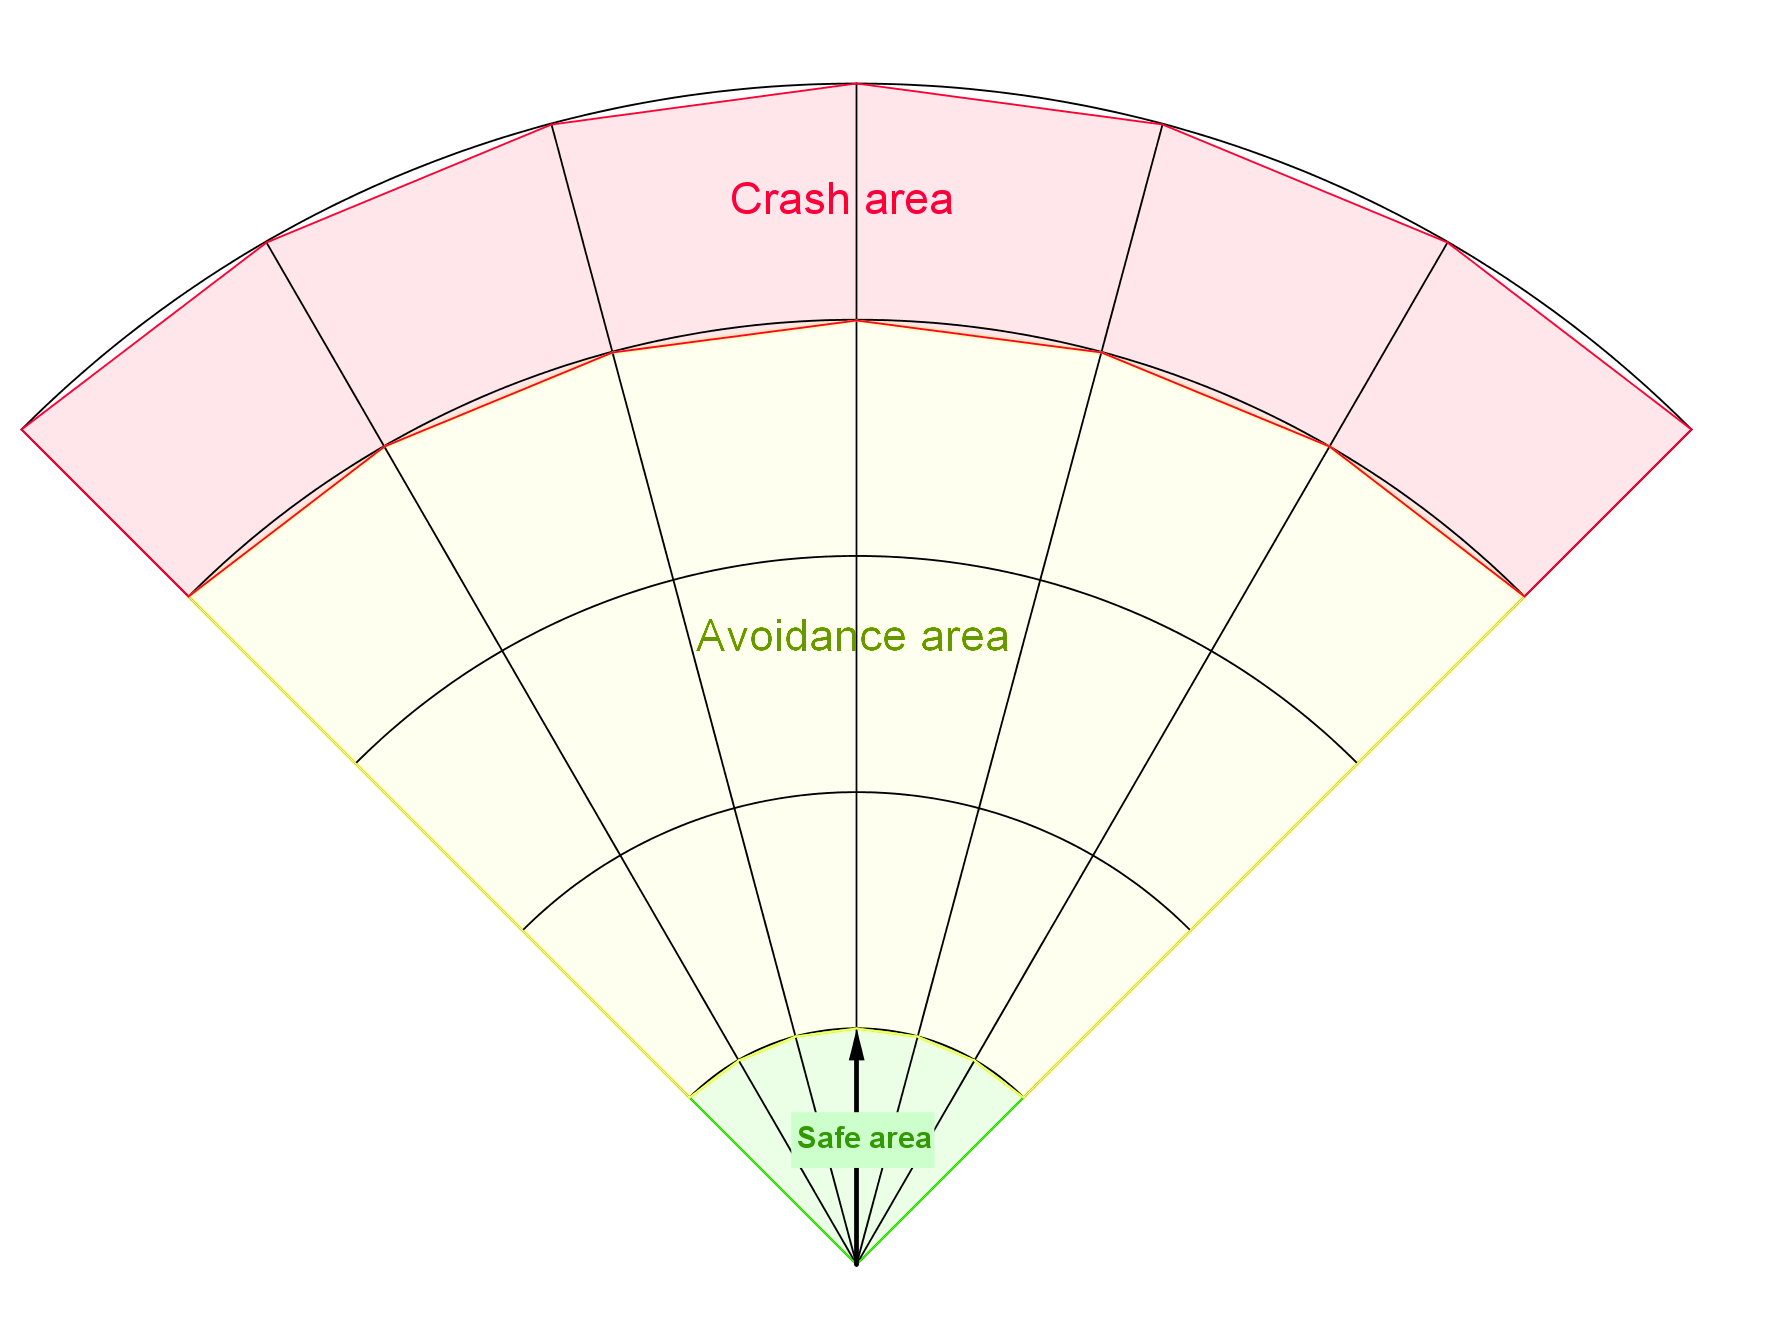
\includegraphics[width=0.9\linewidth]{\FIGDIR/CA006FieldOfViewZones} 
        \caption{Grid Zones.}
        \label{fig:gridZonesMissionControl}
    \end{subfigure}
    \caption{Definitions for \emph{Mission Control Run} (outer loop).}
    \label{fig:definitionsForMissionControlRun}
\end{figure}

\noindent Joining \emph{Avoidance Grid Runs} (fig. \ref{fig:joiningMultipleAGRS})  example portrays \emph{Avoidance Grid Runs} invoked on various \emph{Decision Points} to achieve \emph{Navigation} functionality. The UAS (blue plane) is flying Mission (green numbered waypoints). The \emph{Avoidance Grid} boundary (black dashed line) for each \emph{Decision Point} (UAS position at time $t_i$). Following example of \emph{Navigation} (fig. \ref{fig:missionControlRunActivityDiagram}) run is shown:

\begin{enumerate}
    \item \emph{Mission Start} (fig. \ref{fig:missionExampleWithOAGR}) - UAS at the start of the mission have one \emph{Avoidance Grid} at its position to determine the \emph{Navigation Path} to \emph{Waypoint 2} (goal waypoint). The planned path (red line) is leading directly to \emph{Avoidance Grid} boundary (black dashed line).
    
    \item \emph{Mission End} (fig. \ref{fig:finishedMissionAGR}) - UAS have reached 
    \emph{last waypoint}. All \emph{Avoidance Grid} boundaries (black dashed line) for all \emph{runs} are drawn along flown trajectory. 
    
    \item \emph{Waypoint Reach} (fig. \ref{fig:waypointReachAGR}) - the \emph{waypoint} is inside \emph{Avoidance Grid}, the navigation path (red line) leads directly to \emph{goal waypoint}. (Excessive \emph{Avoidance Grid} boundaries are removed.)
    
    \item \emph{Next Waypoint} (fig. \ref{fig:newtWaypointAGR}) - the new \emph{Goal Waypoint} is selected, the UAS moves to new goal (invoking \emph{Avoidance Grid Runs} when necessary).
    
\end{enumerate}

\begin{figure}[H]
    \centering
    \begin{subfigure}{0.48\textwidth}
        \centering
        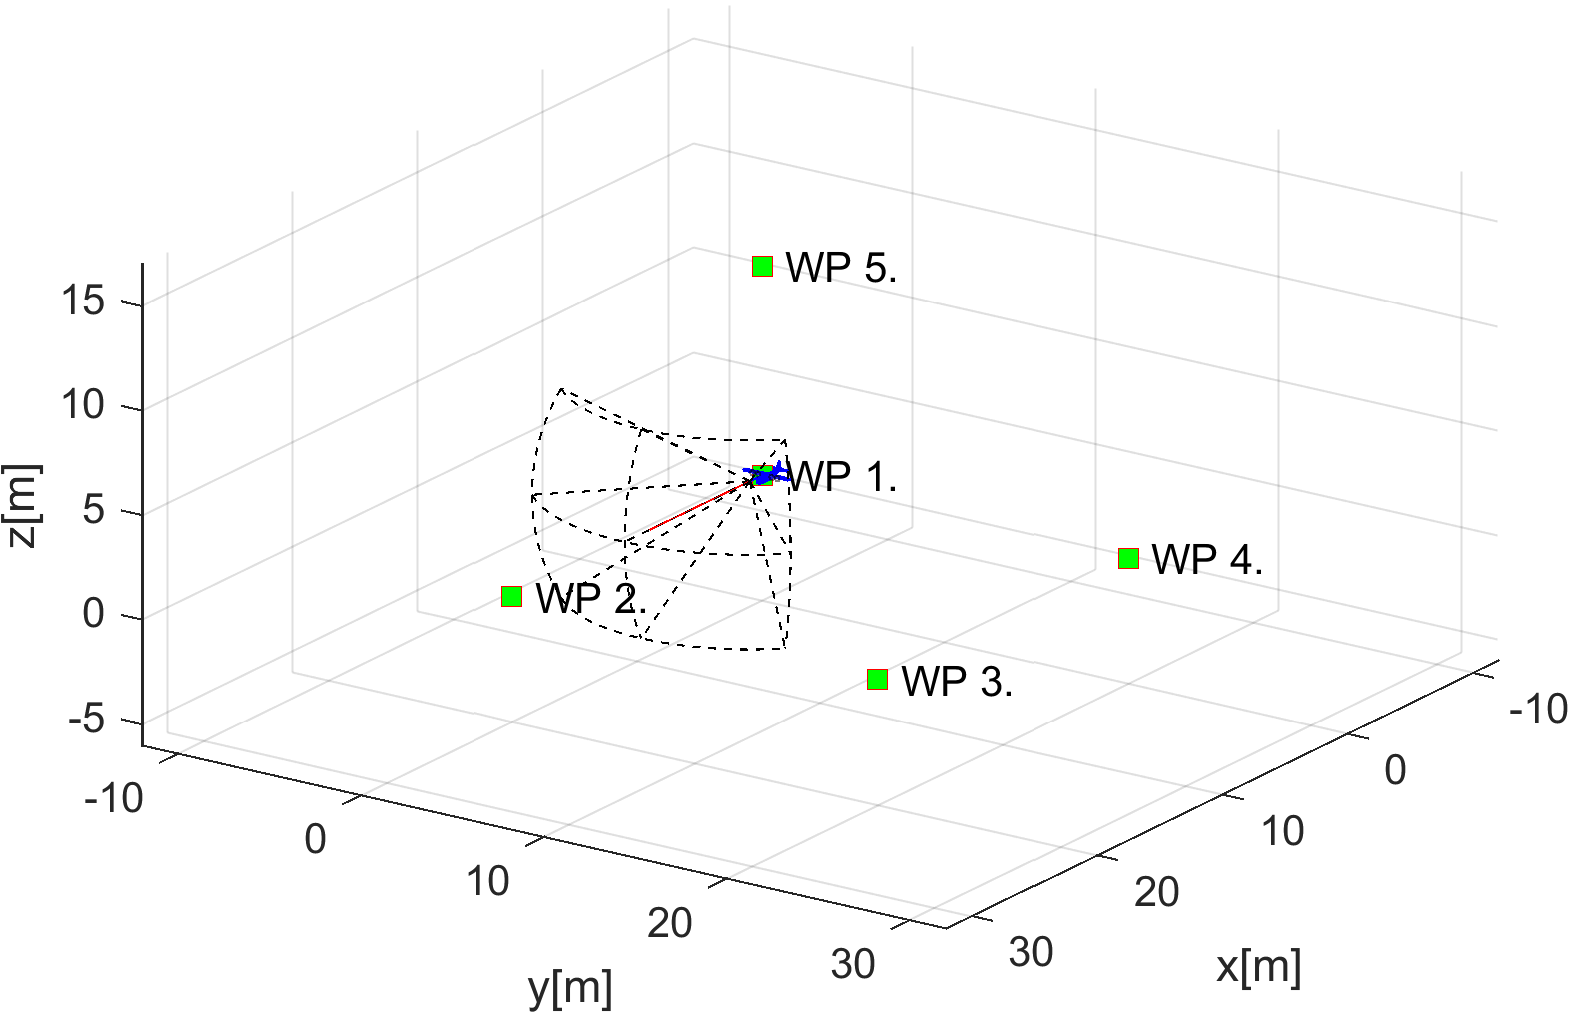
\includegraphics[width=0.9\linewidth]{\FIGDIR/TE042MissionExample}
        \caption{Mission start.}
        \label{fig:missionExampleWithOAGR}
    \end{subfigure}
    \begin{subfigure}{0.48\textwidth}
    	\centering
        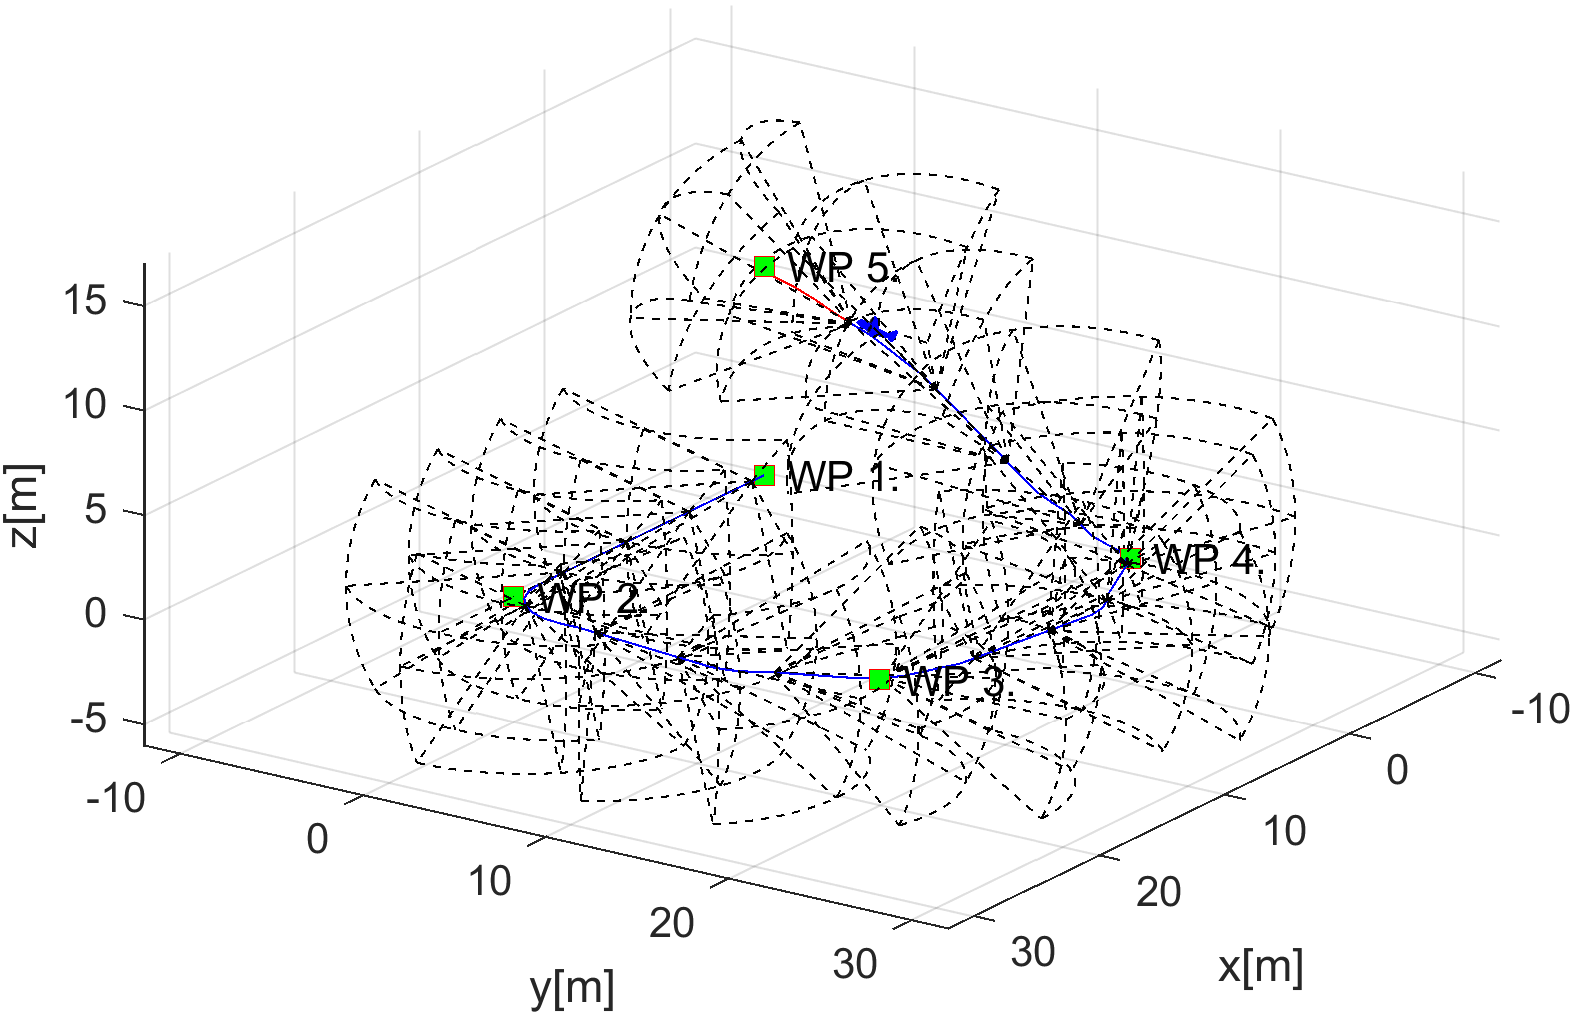
\includegraphics[width=0.9\linewidth]{\FIGDIR/TE043AllDecisionDecisionPoint} 
        \caption{Mission end.}
        \label{fig:finishedMissionAGR}
    \end{subfigure}
    \\
    \centering
    \begin{subfigure}{0.48\textwidth}
        \centering
        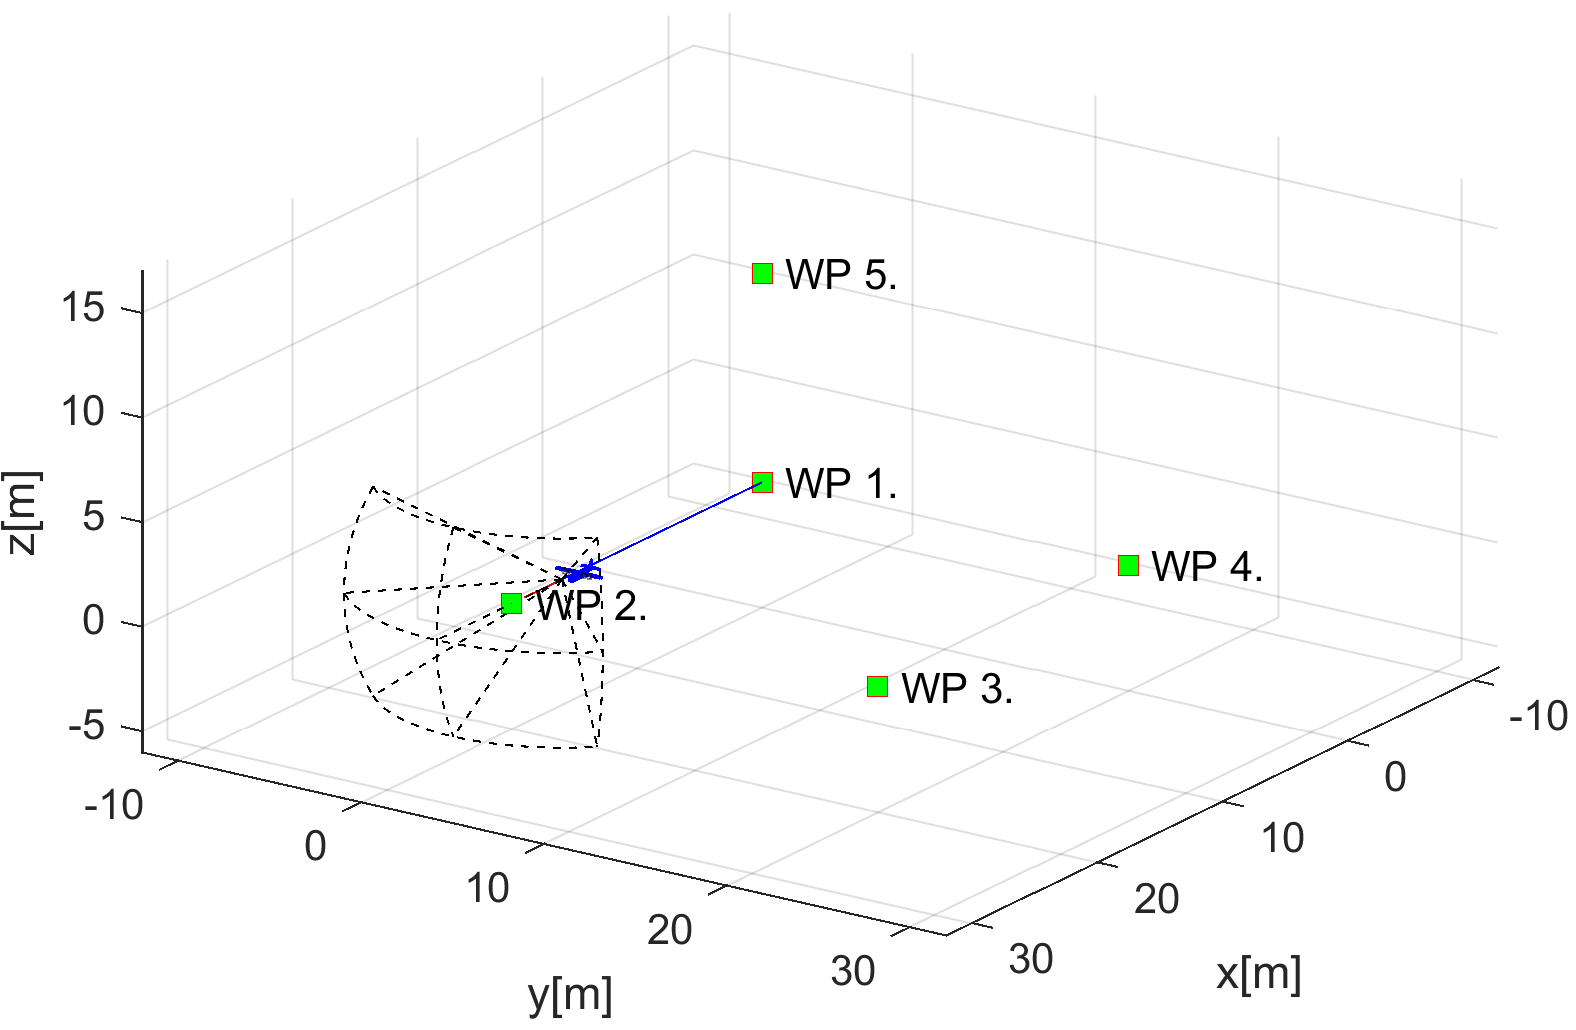
\includegraphics[width=0.9\linewidth]{\FIGDIR/TE044WaypointReach}
        \caption{Waypoint reach.}
        \label{fig:waypointReachAGR}
    \end{subfigure}
    \begin{subfigure}{0.48\textwidth}
    	\centering
        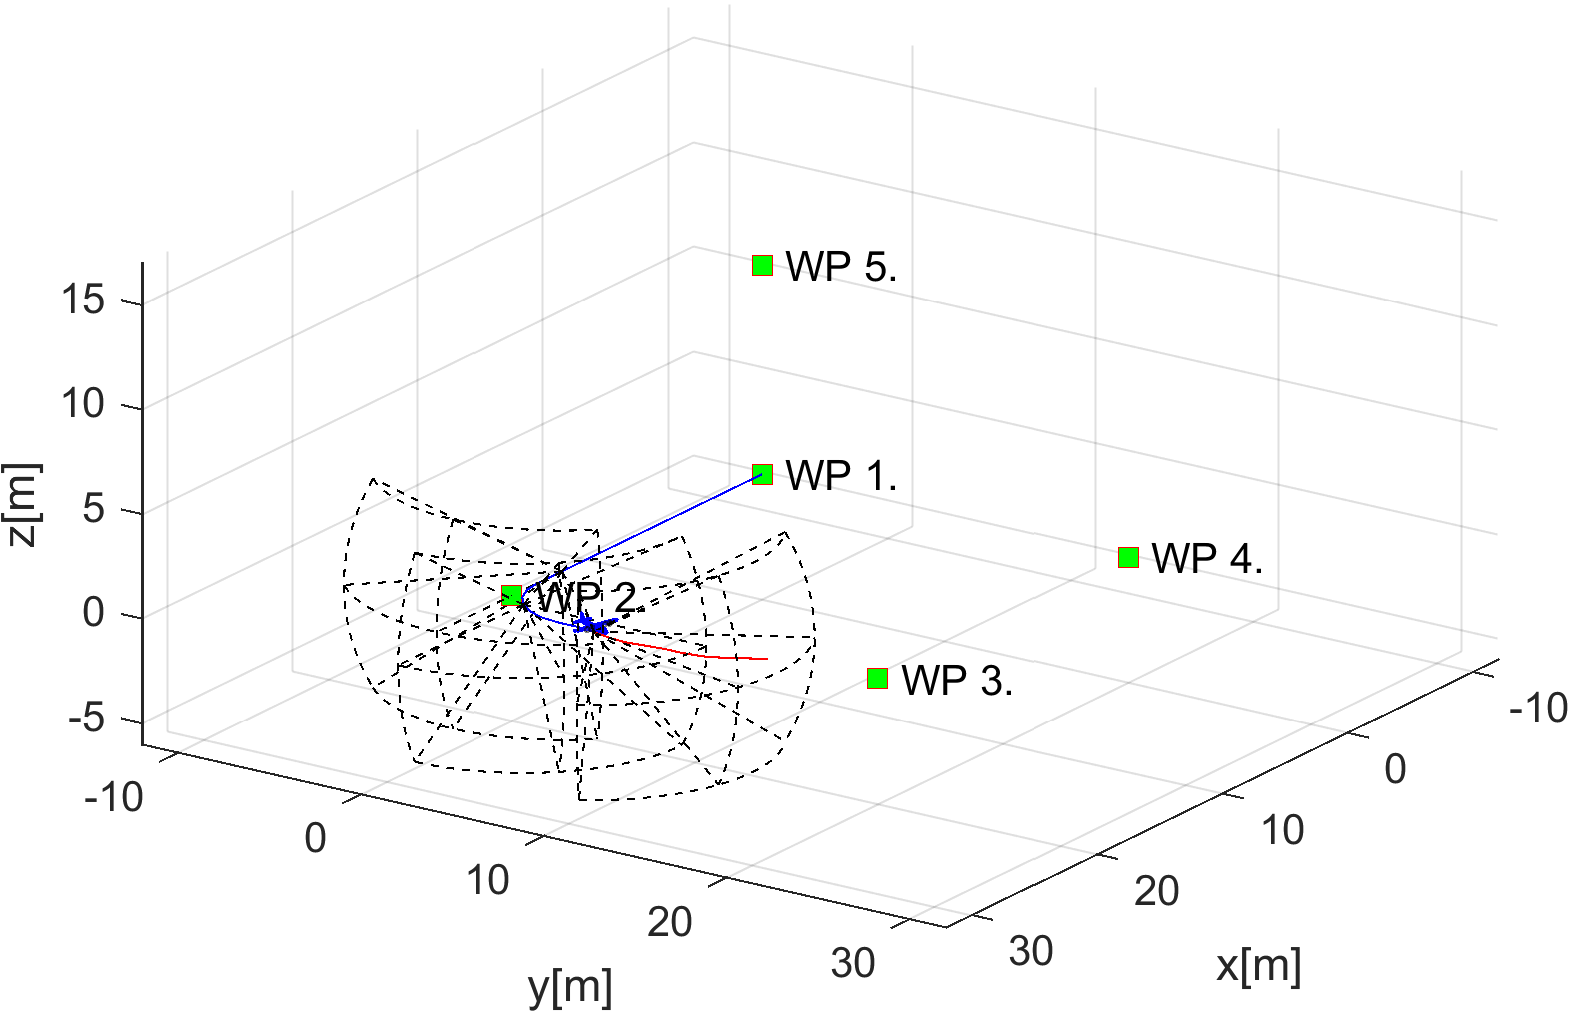
\includegraphics[width=0.9\linewidth]{\FIGDIR/TE045NewWaypointSetup} 
        \caption{Next waypoint.}
        \label{fig:newtWaypointAGR}
    \end{subfigure}
    \caption{Joining multiple \emph{Avoidance Grid Runs} for achieve Navigation.}
    \label{fig:joiningMultipleAGRS}
    
\end{figure}
    

\newpage
\paragraph{General Concept:}\footnote{Mission Control Run Function Implementation: \url{RuleEngine/MissionControl/MissionControl.m::runOnce(.)}} The \emph{General Concept} is taken from  \cite{sabatini2014navigation,Sabatini2014}, consisting from following main modules:
\begin{enumerate}
    \item \emph{Navigation Loop} - module responsible for \emph{Navigation} providing \emph{Goal Waypoint}.
    
    \item \emph{Data Fusion} (background in sec. \ref{s:sensorFusion}) - module responsible for \emph{Surveillance Data Feed}.
    
    \item \emph{Situation Assessment} - module responsible for \emph{UAS Safety Evaluation}. 
    
    \item \emph{Avoidance Run} (background in sec. \ref{s:aviudabceGridRun}) responsible for \emph{Avoidance Path} selection.    
\end{enumerate}


\begin{figure}[H]
    \centering
    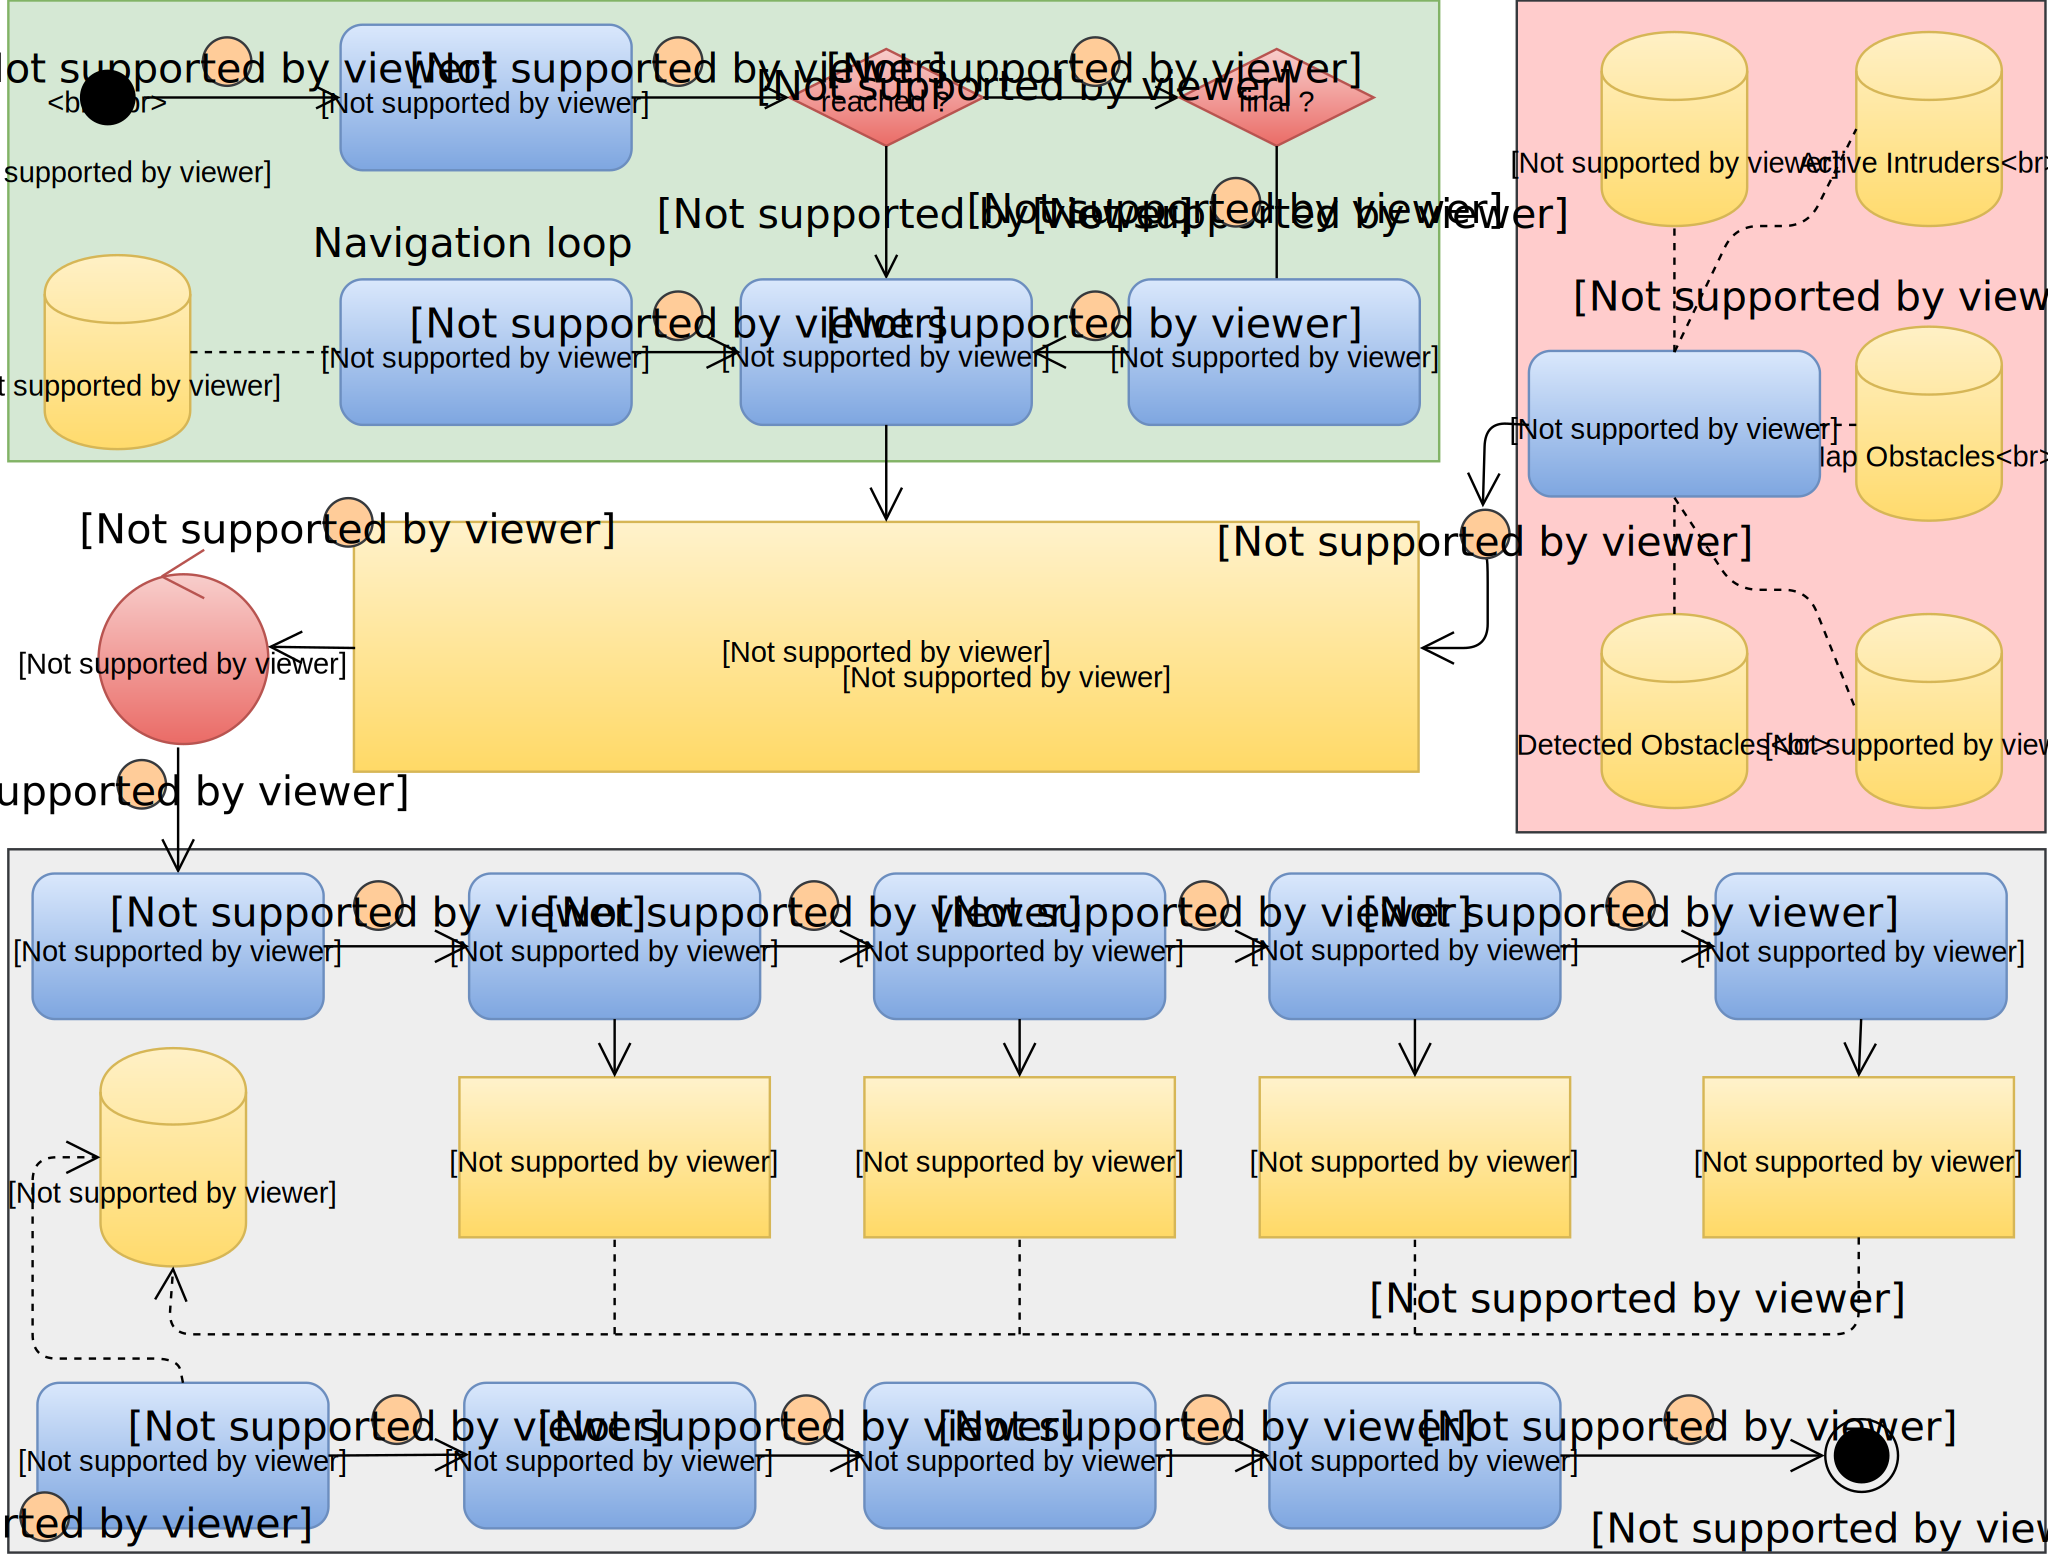
\includegraphics[width=\linewidth]{\FIGDIR/TE026AvoidanceAlgorithmMainLoopRun}
    \caption{Mission control run activity diagram.}
    \label{fig:missionControlRunActivityDiagram}
\end{figure}

\noindent The main changes to \emph{Navigation architecture} are given in \emph{Mission Control Run} activity diagram (fig. \ref{fig:missionControlRunActivityDiagram}):

\begin{enumerate}
    \item \emph{Situation Assessment} - added event-based mode switching control. 
   
    \item \emph{Avoidance Run} - added hierarchical evaluation for \emph{Avoidance Path} selection. Prioritizing threat avoidance according to a type. 
\end{enumerate}

\noindent The \emph{Operation Mode} is introduced, based on \emph{Situation assessment} and \emph{Triggering Events} one of following modes are selected in \emph{Avoidance Run}:

\begin{enumerate}
    \item \emph{Navigation Mode} - the \emph{UAS} is navigating through \emph{Airspace} following \emph{cost effective patterns} and obeying \emph{Airspace Authority} (UTM). The \emph{Navigation Grid} is a instance of \emph{Avoidance Grid} (sec. \ref{s:AvoidanceGrid}) with initialized \emph{Navigation Reach Set} (ex. \emph{Harmonic Reach Set Approximation} (sec. \ref{s:harmonicReachSet})).
    
    \item \emph{Emergency Avoidance Mode} - the \emph{UAS} is \emph{threatened} by obstacle, intruder, hard constraint or \emph{soft constraint}, the \emph{UAS} is navigating through \emph{Airspace} following \emph{safe avoidance patterns} and \emph{minimizing the impact} of possible damages. The \emph{Avoidance Grid} is term used for \emph{Emergency Avoidance Mode}. The \emph{Avoidance Reach Set Approximation} is initialized in \emph{Avoidance Grid} (ex. \emph{Chaotic Reach Set Approximation} (sec. \ref{s:chaoticReachSet}))
\end{enumerate}

\begin{note}
    Depending on \emph{Operation Mode} the pair of \emph{Avoidance Grid} and \emph{Reach Set} is selected in \emph{Avoidance Run} part.
    
    
    The \emph{Navigation Grid} and \emph{Avoidance Grid} shares the space segmentation pattern, therefore the \emph{Data Fusion} (sec. \ref{s:sensorFusion}) needs to be evaluated only once for both grids. 
\end{note}



\paragraph{Decision Time Frame ($[t_i,t_{i+1}[$):} The \emph{Mission Control Run} is executed for \emph{Decision Time Frame} bounded to the \emph{period} of the \emph{UAS executed movement} (fig. \ref{fig:AvoidanceFrameworkConceptNew}).

The \emph{UAS System} (sec. \ref{s:UASNonlinearModel}) controlled by \emph{Movement Automaton Implementation} (sec. \ref{s:movementAutomatonDefinition}) \emph{Planned Movements} can be changed at any time. The real impact on control is shown after the \emph{actual movement} is executed. 

\begin{note}
    For our \emph{Movement Automaton Implementation} movements the average \emph{movement duration} is \emph{1/velocity second} (tab. \ref{tab:movements1}, \ref{tab:movements2}).
\end{note}

The \emph{Decisions} are made based on \emph{system} state in \emph{current} time-frame started at $t_i$ for \emph{next} time frame starting at $t_{i+1}$.

\begin{note}
    Because the \emph{Decision Delay} is crucial in \emph{Avoidance System} it is beneficial to have \emph{short time movements}. On the other hands, the \emph{length and duration  of movements} is impacting \emph{Reach Set Complexity}. The proper construction of movement automaton is greatly impacting overall \emph{approach performance}.
\end{note}

\paragraph{Initialization:} The \emph{UAS} is going to solve a problem for \emph{Rules of the Air} (eq. \ref{eq:rulesOfTheAir}). Using control scheme (fig. \ref{fig:AvoidanceFrameworkConceptNew}) with given \emph{Sensors}:

\begin{equation}
    Sensors = \{LiDAR,ADS-B\}
\end{equation}

\noindent The sensors obstacle assessment into avoidance grid is outlined for static obstacles in (sec. \ref{s:staticObstacles}) and for moving obstacles in (sec. \ref{s:intruders}.)

\noindent The \emph{Data Fusion Procedure} is given as follow:
\begin{equation}
    DataFusion = \{Rating Based Data Fusion \quad (sec. \ref{s:sensorFusion})\}
\end{equation}

Then the \emph{UAS system} (sec. \ref{s:UASNonlinearModel}) with \emph{Movement Automaton Implementation} (sec. \ref{s:movementAutomatonDefinition}) with empty movement buffer:

\begin{equation}
    Movement Buffer = \{\}
\end{equation}

\noindent The \emph{Avoidance Grids} for both \emph{Operation Modes} are created with \emph{identical space segmentation}. The \emph{Reach Set Approximations} are loaded based on initial \emph{UAS State} at decision time $0$. The \emph{Reach Set Approximation} is always selected based on \emph{UAS System State}. The initial \emph{Operation Mode} is set up as \emph{Navigation}. The initialization is summarized like follow:

\begin{equation}
    \begin{aligned}
    Avoidance Grid(0) &= \{UAS.position(0),AvoidanceReachSet(UAS.ReachSet)\}\\
    Navigation Grid (0) &= \{UAS.position(0), NavigationReachSet(UAS.ReachSet)\}\\
    Operation Mode &= Navigation
    \end{aligned}
\end{equation}

The \emph{Mission} is set up as a set of \emph{ordered waypoints}. The \emph{initial goal waypoint} is \emph{first waypoint}. The initialization is summarized like follow:

\begin{equation}
    \begin{aligned}
    Mission &= \{Waypoint_1 \dots  Waypoint_n\}\\
    Goal Waypoint &= Mission.waypoint_1\\
    Last Waypoint &= Mission.waypoint_n\\
    \end{aligned}
\end{equation}

The \emph{actual threats} are set as empty sets for \emph{decision time} $t_i=0$:
\begin{equation}
    \begin{aligned}
    obstacles &= \{\}, intruders = \{\}, hard Constraints = \{\}, soft Constraints = \{\}\\
    \end{aligned}
\end{equation}



\paragraph{Navigation Loop (1\textsuperscript{st}-3\textsuperscript{rd} step):} The purpose of \emph{Navigation Loop} is to select proper \emph{Goal Waypoint} from \emph{Mission} (sec. \ref{s:mission}). If \emph{last waypoint} have been reached the \emph{Landing Procedure} will be initiated and \emph{Mission Control Run} Ends.

\noindent First start with definition of \emph{waypoint reach condition} (def. \ref{def:waypointReachCondition}) and \emph{Unreachable waypoint} (def. \ref{def:unreachable Waypoint}).

\newpage
\begin{definition}{Waypoint Reach Condition}\label{def:waypointReachCondition} for \emph{current} decision time $t_i$ for \emph{UAS} position and current \emph{Goal Waypoint} is satisfied only if:

\begin{multline}\label{eq:waypointReachCondition}
    distance(UAS.position(t_i),GoalWaypoint(t_i)) \\\le \\2 \times \max \left\{length(movement):\forall movement\in MovementSet\right\}
\end{multline}

    \begin{note}
        The movements in our solution have \emph{uniform length} of \emph{1 m} (tab. \ref{tab:movements1}, \ref{tab:movements2}), therefore the waypoint reach condition is satisfied when \emph{distance to goal waypoint} is lesser than 2 m. The maximal movement length has impact on \emph{navigation/avoidance} precision.
    \end{note}
\end{definition}

\begin{definition}{Unreachable Waypoint}\label{def:unreachable Waypoint}. The \emph{Goal Waypoint} is evaluated as unreachable in decision time $t_i$ when \emph{Avoidance Grid Run} (alg. \ref{alg:FindBestPathAvoidanceGrid}) cannot find the \emph{navigation/avoidance path} leading to it.

\noindent Formally: The \emph{Avoidance/Navigation Grid} has range defined as \emph{final layer distance}. When the \emph{Goal Waypoint} is in  \emph{range} of \emph{Grid}:

\begin{equation}
    Grid(t_i).range \ge distance(UAS.position(t_i),GoalWaypoint(t_i))
\end{equation}

\noindent and following condition is satisfied:

\begin{multline}\label{eq:unreachableWaypoint}
    \forall cell_{i,j,k}\in Grid(t_i) \not\exists cell_{i,j,k}. Reachable == true \wedge\dots  \\\dots\wedge distance(cell_{i,j,k}, Goal Waypoint(t_i)) \le\dots \\ \dots\le 2 \times \max \left\{length(movement):\forall movement\in MovementSet\right\}
\end{multline}

\noindent The \emph{Goal Waypoint} is unreachable.

\end{definition}

Then the \emph{Navigation Loop} is invoked  every \emph{decision time} $t_i$, \emph{Mission Control Run} (fig. \ref{fig:missionControlRunActivityDiagram}), it is described as sequence of following steps:

\begin{itemize}
    \item[\textbf{1\textsuperscript{st}}] \textbf{Check Waypoint Reach Condition} - the \emph{UAS position} for given \emph{time frame} $t_i$ is checked under condition (eq. \ref{eq:waypointReachCondition}).  If condition is met continue with 2\textsuperscript{nd} step otherwise continue with 3\textsuperscript{rd} step.

    \item[\textbf{2\textsuperscript{nd}}] \textbf{Set Next Waypoint} - until following condition is met:
    \begin{equation*}
        Goal Waypoint == Last Waypoint    
    \end{equation*}
    Set next goal waypoint like follow:
    \begin{equation*}
        Goal Waypoint = Mission.get Next Waypoint()
    \end{equation*}
    Otherwise enforce \emph{Landing sequence} (Out of Scope).
        
    \item[\textbf{3\textsuperscript{rd}}] \textbf{Trajectory Prediction} - the \emph{Movement Buffer} is loaded with planned movements from \emph{Movement Automaton}. The \emph{future trajectory} is predicted according to (eq. \ref{eq:ourTrajectoryImplementation}):
    \begin{multline*}
        Predicted Trajectory = \\Trajectory(state=UAS.state(t_i),buffer=future Movements)
    \end{multline*}
\end{itemize}

\noindent The \emph{Predicted Trajectory} is used in 5\textsuperscript{th} step \emph{Situation Assessment}.

\paragraph{Data Fusion (4\textsuperscript{th} step)} The \emph{Data Fusion} (sec. \ref{s:sensorFusion}) in this context is \emph{Threat Sets} preparation for \emph{Avoidance Run}. It is depending on values of \emph{Boolean values} defined in (tab. \ref{tab:defuzificationRatings}) for \emph{threat} classification.

\begin{note}
    Avoidance Grid`s Data fusion (sec. \ref{s:sensorFusion}) is run in 7\textsuperscript{th}- 10\textsuperscript{th} step (fig. \ref{fig:missionControlRunActivityDiagram}). 
\end{note}

The \emph{static obstacles} source is from \emph{LiDAR} scan received at least at beginning of current \emph{decision frame} $t_i$:

\begin{equation*}
        obstacles=LiDAR.scan(UAS.position(t_i))
\end{equation*}

The \emph{intruders} source are valid \emph{active intruders notifications} received from ADS-B In positioned to \emph{future expected positions} at \emph{decision time} $t_{i+1}$:

\begin{equation*}
        intruders=ADS-B.get Active Intruders(t_{i+1})
\end{equation*}

\begin{note}
    The \emph{Intruders} needs to be predicted for the next decision time-frame starting at time $t_{i+1}$ Due their mobility.
\end{note}

\noindent The \emph{hard/soft constraints} are obtained from \emph{Information Sources} and the area of next decision time $t_{i+1}$ \emph{Avoidance Frame} is used as space parameter in search. The sets of hard and soft constraints are obtained in following manner:

\begin{equation*}
    hard Constraints= Information Sources.fuse(Avoidance Grid(t_{i+1}))
\end{equation*}

\begin{equation*}        
        soft Constraints=Information Sources.fuse(Avoidance Grid(t_{i+1}))
\end{equation*}

\noindent The results of \emph{Data Fusion} threats set preparation are used in next step.


\paragraph{Invoke Navigation/Avoidance based on Situation Assessment (5\textsuperscript{th}-6\textsuperscript{th} step):} The \emph{deciding events} depending on \emph{Trajectory Prediction} ($3^{rd}$ step) and \emph{Data Fusion} ($4^{th}$ step) (fig. \ref{fig:missionControlRunActivityDiagram}) are following:

\begin{enumerate}
    \item \emph{General Events} are \emph{triggered} regardless \emph{Operation Mode}. They are considered after \emph{specific mode events} are handled and \emph{Navigation/Avoidance Grid} is selected:
    \begin{enumerate}[a.]
        \item \emph{Empty Movement Buffer} ($Movement Buffer = \varnothing$) - if there is no movement in \emph{Movement buffer} to be executed (from 3\textsuperscript{rd} step: Load Trajectory), the \emph{Avoidance Run} is enforced to run with \emph{Navigation/Avoidance Reach Set Approximation} to generate new path.
        
        \item \emph{Waypoint Reached} (2\textsuperscript{nd} step) - the \emph{Navigation Loop} run is forced to set goal \emph{Goal Waypoint}. If \emph{last waypoint} from \emph{Mission} (sec. \ref{s:mission}) the \emph{Landing Procedure} is enforced.
        
        \item \emph{Waypoint Unreachable} - this type of event is very situations based. The \emph{Waypoint Reachibility} (assumption. \ref{ass:reachableWaypoints}) has not been relaxed, therefore this event is not properly handled in approach. The \emph{implementation} considers \emph{selecting next waypoint in mission} as a goal waypoint of \emph{first waypoint} if \emph{unreached/unreachable waypoints} are exhausted. 
    \end{enumerate}
    
    \item \emph{Navigation Mode Events} are triggered if \emph{Operation Mode} is set as \emph{Navigation}:
    \begin{enumerate}[a.]
        \item \emph{Empty Navigation Grid} ($|threats| = 0$) - if \emph{movement buffer} contains at least one \emph{movement}, the \emph{Avoidance Run} is omitted. The \emph{Operation Mode} stays in \emph{Navigation Mode}.
        
        \item \emph{Collision Case Resolution} ($|ActiveCollisionCases| > 0$) - there is new/active \emph{Collision Case} (sec. \ref{sec:collisionCase}), the \emph{Navigation Reach Set Approximation} trajectories will be constrained according to  active \emph{Collision Case(s)} requirements. If there exists at least one \emph{Reachable} avoidance path, the \emph{Operation Mode} will remain \emph{Navigation}. If there is no  \emph{Reachable} avoidance path, the \emph{Operation Mode} switches to \emph{Emergency Avoidance}.
        
        \item \emph{Static Obstacle Detection} ($LiDAR.Hits > threshold$) - if \emph{static obstacle set} contains at least one \emph{detected obstacle} (sec. \ref{s:detectedObstacles}) intersecting with \emph{Navigation  grid} the \emph{Operation Mode} will be \emph{switched} to \emph{Emergency Avoidance Mode}.
        
        \item \emph{Intruder Detection} ($intruders> 0$) - if \emph{active intruders set} contains at least one \emph{intruder} which expected impact area (intersection models (sec. \ref{s:intruderBehaviourPrediction})) \emph{Navigation  grid} the \emph{Operation Mode} will be \emph{switched} to \emph{Emergency Avoidance Mode}.
        
        \item \emph{Hard or Soft Constraint Occurrence} ($|hard Constraints|$ $>$ $0$ $\vee$ $|soft Constraints|$ $>$ $0$) - if \emph{hard/soft constraint set} contains at least one \emph{constraints} which intersects (static constraints (sec. \ref{s:virtualConstraints}), moving constraints (sec. \ref{s:MovingVirtualConstraints})) \emph{Navigation  grid} the \emph{Operation Mode} will be \emph{switched} to \emph{Emergency Avoidance Mode}.
    \end{enumerate}
    
    \item \emph{Emergency Avoidance Events} are triggered if \emph{Operation Mode} is set as \emph{Emergency Avoidance}:
    \begin{enumerate}[a.]
        \item \emph{Empty Avoidance Grid} ($|threats| = 0$) - if there is no \emph{detectable} threat, the remainder of \emph{avoidance path} is removed from \emph{Movement Buffer}. The \emph{Operation Mode} is switched to \emph{Navigation} and new \emph{navigation path} is selected. 
    \end{enumerate}
\end{enumerate}



\begin{itemize}
    \item[\textbf{5\textsuperscript{th}}] \textbf{Situation Assessment} - if there is any flag raised by \emph{Event Triggers}, there is an \emph{avoidance situation}.
    
    The \emph{Event Triggers} describe complex \emph{Operation Mode} switching. The simplified principle is following: \emph{If UAS is in Emergency Avoidance Mode Always Invoke Avoidance Run. If UAS is in Navigation Mode Invoke Only if Necessary}.
    
    If there was event trigger continue with 7\textsuperscript{th} step, otherwise wait for \emph{next decision time} $t_{i+1}$, execute movement and continue with 1\textsuperscript{st} step.
    
    \item[\textbf{6\textsuperscript{th}}] \textbf{Invoke Navigation/Avoidance} depending on the \emph{Operation Mode} the \emph{Reach Set/Grid} pair is selected. The future $state(t_{i+1})$ in next decision frame $t_{i+1}$ is necessary for Grid/Reach Set initialization. The \emph{next decision frame initial state} is obtained by \emph{prediction}:
    
    \begin{equation*}
        state(t_{i+1}) =  Trajectory(state(t_i),current Movement)
    \end{equation*}
    
    The \emph{Reach Set Approximation} is loaded based on \emph{mode} and $state(t_{i+1})$. The \emph{Grid} is initialized as $Free(t_{i+1})$ (eq. \ref{eq:freeDataFusion}) for all cells.
\end{itemize}



\paragraph{Avoidance Run (7\textsuperscript{th}-15\textsuperscript{th} step):} The \emph{Avoidance Run} goal is to obtain \emph{Path} represented as \emph{Trajectory}(state($t_{+1}$,MovementBuffer)) (eq. \ref{eq:ourTrajectoryImplementation}) from \emph{Navigation/Avoidance Grid} and associated \emph{Navigation/Avoidance Reach Set Approximation}.

If the \emph{Operation Mode} is set as \emph{Navigation Mode} the algorithm continues with 11\textsuperscript{th} step. Otherwise the \emph{Avoidance Grid Space Assessment} is run multiple times to obtain $Reachable(t_{i+1})$ (eq. \ref{eq:ReachableDataFusion}). The \emph{Threat Data} obtained from 4\textsuperscript{th} step are used. 

\begin{itemize}
    
    \item[\textbf{7\textsuperscript{th}}] \textbf{Apply Obstacles} - The \emph{Space assessment} (tab. \ref{tab:defuzificationRatings}) for \emph{Avoidance Grid} is calculated  with following threat modification:
    
    \begin{equation*}
        intruders = \varnothing, soft Constraints = \varnothing, hard Constraints = \varnothing
    \end{equation*}
    
    The \emph{Find Best Path} (alg. \ref{alg:FindBestPathAvoidanceGrid}) is applied, the resulting \emph{avoidance path} is labeled as \emph{Obstacle Avoidance Path}.
  
    \item[\textbf{8\textsuperscript{th}}] \textbf{Apply Intruders} - The \emph{Space assessment} (tab. \ref{tab:defuzificationRatings}) for \emph{Avoidance Grid} is calculated  with following threat modification:
    
    \begin{equation*}
        soft Constraints = \varnothing, hard Constraints = \varnothing
    \end{equation*}
    
    The \emph{Find Best Path} (alg. \ref{alg:FindBestPathAvoidanceGrid}) is applied, the resulting \emph{avoidance path} is labeled as \emph{Intruders Avoidance Path}.
    
    \item[\textbf{9\textsuperscript{th}}] \textbf{Apply Hard Constraints} - The \emph{Space assessment} (tab. \ref{tab:defuzificationRatings}) for \emph{Avoidance Grid} is calculated  with following threat modification:
    
    \begin{equation*}
        hard Constraints = \varnothing
    \end{equation*}
    
    The \emph{Find Best Path} (alg. \ref{alg:FindBestPathAvoidanceGrid}) is applied, the resulting \emph{avoidance path} is labeled as \emph{Hard Constraint Avoidance Path}.
    
    \item[\textbf{10\textsuperscript{th}}] \textbf{Apply Soft Constraints} - The \emph{Space assessment} (tab. \ref{tab:defuzificationRatings}) for \emph{Avoidance Grid} is calculated  without any modification.
    
    The \emph{Find Best Path} (alg. \ref{alg:FindBestPathAvoidanceGrid}) is applied, the resulting \emph{avoidance path} is labeled as \emph{Soft Constraints Avoidance Path}.
    
    \begin{note}
        The 7\textsuperscript{th} to 10\textsuperscript{th} steps are code-optimized for efficient calculation.
    \end{note}
    
    \item[\textbf{11\textsuperscript{th}}] \textbf{Select Path} -  based on \emph{Operation Mode} the \emph{Navigation/Avoidance Path} is selected.
    
    The \emph{Navigation Path} for \emph{Navigation Mode} is selected by standard \emph{Find Best Path} (alg. \ref{alg:FindBestPathAvoidanceGrid}) procedure. The \emph{Navigation Reach Set Approximation} can be constrained by \emph{Rule Engine} (fig. \ref{fig:RuleEngineInstanceLevels}).
    
    The \emph{Avoidance Path} for \emph{Emergency Avoidance Mode} is selected from \emph{Collected Avoidance Paths} with following priority:
    \begin{itemize}
        \item[1.] \emph{Soft Constraints Avoidance Path} - if exists continue with 12\textsuperscript{th} step, if does not exist try to select:
        
        \item[2.] \emph{Hard Constraints Avoidance Path} - if exists continue with 12\textsuperscript{th} step, if does not exist try to select:
        
        \item[3.] \emph{Intruders Avoidance Path} - if exists continue with 12\textsuperscript{th} step, if does not exist try to select:
        
        \item[4.] \emph{Obstacle Avoidance Path} - continue with 12\textsuperscript{th} step.
    \end{itemize}
    \begin{note}
        The \emph{Waypoint Reachibility} (assumption \ref{ass:reachableWaypoints}) is weakened to the point that it is necessary for waypoint to be \emph{Reachable} only in static obstacle environment. The \emph{Constrained} and \emph{Occupied} spaces are shrunk in following matter to increase UAS survival chances. There are following relaxations with their conditions:
        \begin{itemize}
            \item[1.] \emph{Soft Constraint Relaxation} - they are breakable by default.  This kind of situation is allowed to happen under any circumstances. 
            
            \item[2.] \emph{Hard Constraints Relaxation} - they can be broken in case of emergency (airspace constraints) or UAS robust build (Weather Constraints). This kind of situation is allowed under very specific conditions depending on \emph{broken constraint} severity.
            
            \item[3.] \emph{Intruder Occupied Space Relaxation} - this can be broken if and only if there is guarantee the Intruder dynamic and navigation algorithm allows to avoid \emph{Collision} with UAS. This relaxation should be used as \emph{the last resort}.
        \end{itemize}
    \end{note}
    
    \item[\textbf{12\textsuperscript{th}}] \textbf{Load Movements} - the \emph{Movement Buffer} is flushed for \emph{future decision times} $t_{i+1}, \dots, t_{i+k}$. The \emph{Navigation/Avoidance Path} movements are pushed into \emph{Movement Buffer} instead. The \emph{executed movement} for \emph{decision time} $t_i$ remains (because its executed at this time point).
    
    \item[\textbf{13\textsuperscript{th}}] \textbf{Set Next Decision} - the \emph{next decision point} is set depending on circumstances:
    \begin{itemize}
        \item[1.] Navigation Mode (no active collision cases) - \emph{Decision Point} is set as point before \emph{UAS} enters into \emph{Crash Zone} (fig. \ref{fig:gridZonesMissionControl}) in \emph{Navigation Grid}.
        
        \item[2.] \emph{Navigation Mode (at least one active collision case)} - \emph{Decision Point} is set after \emph{next movement execution}. Current decision point $UAS.Position(t_i)$, next decision point $UAS.Position(t_{i+1})$.
        
        \item[3.] \emph{Emergency Avoidance Mode (any circumstances)} - \emph{Decision Point} is set after \emph{next movement execution}. Current decision point $UAS.Position(t_i)$, next decision point $UAS.Position(t_{i+1})$.
    \end{itemize}
    
    \item[\textbf{14\textsuperscript{th}}] \textbf{Execute Movement} - the \emph{First Movement} from \emph{Movement Buffer} is loaded to be executed in decision time frame $[t_{i+1}, t_{i+2}[$. 
    
    \item[\textbf{15\textsuperscript{th}}] \textbf{Finish Avoidance Run} - if the \emph{UAS} is flying, continue with 1\textsuperscript{st} step. 
\end{itemize}

\paragraph{Decision Frame:} The \emph{mission control run} (fig. \ref{fig:missionControlRunActivityDiagram}) describes overall process in \emph{sequence}. The \emph{orchestration overview} is given in (fig. \ref{fig:misisonControlRunOrchestrationDiagram}).

The key idea is to explain what happen in one \emph{decision frame}. The \emph{mission control run} is implemented as multi-thread application which sends the signals between threads. Each thread is semi-independent process with forced synchronization on \emph{decision frame switch}.

\noindent The notable threads and their roles \& responsibilities are summarized like follow:
\begin{itemize}
    \item[1.] \emph{Sensor Fusion} - responsible for processing real time sensor array (sec. \ref{s:SensorFusionDefinition}). The output is partial known world assessment (sec. \ref{s:KnownWorld}). An \emph{obstacle detection} and \emph{intruder detection} events can be risen by this thread. 
    
    \item[2.] \emph{Data Fusion} - responsible for enhancing data from \emph{sensor fusion} by mixing data originating from \emph{information sources} (sec. \ref{s:dataFusionDefinition}). The information sources used in this work contains constraints originating from \emph{geo-fencing}, \emph{weather}, \emph{airspace restrictions}. This thread is delayed by \emph{sensor fusion}. A \emph{data fusion procedure} strongly depends on \emph{operational space context} (controlled/non-controlled airspace). The output of \emph{data fusion} is full \emph{known world assessment} (sec. \ref{s:KnownWorld}, \ref{s:sensorFusion}). The \emph{UTM-related} and \emph{constraint related} events can arise from \emph{data fusion}.
    
    
\begin{figure}[H]
    \centering
    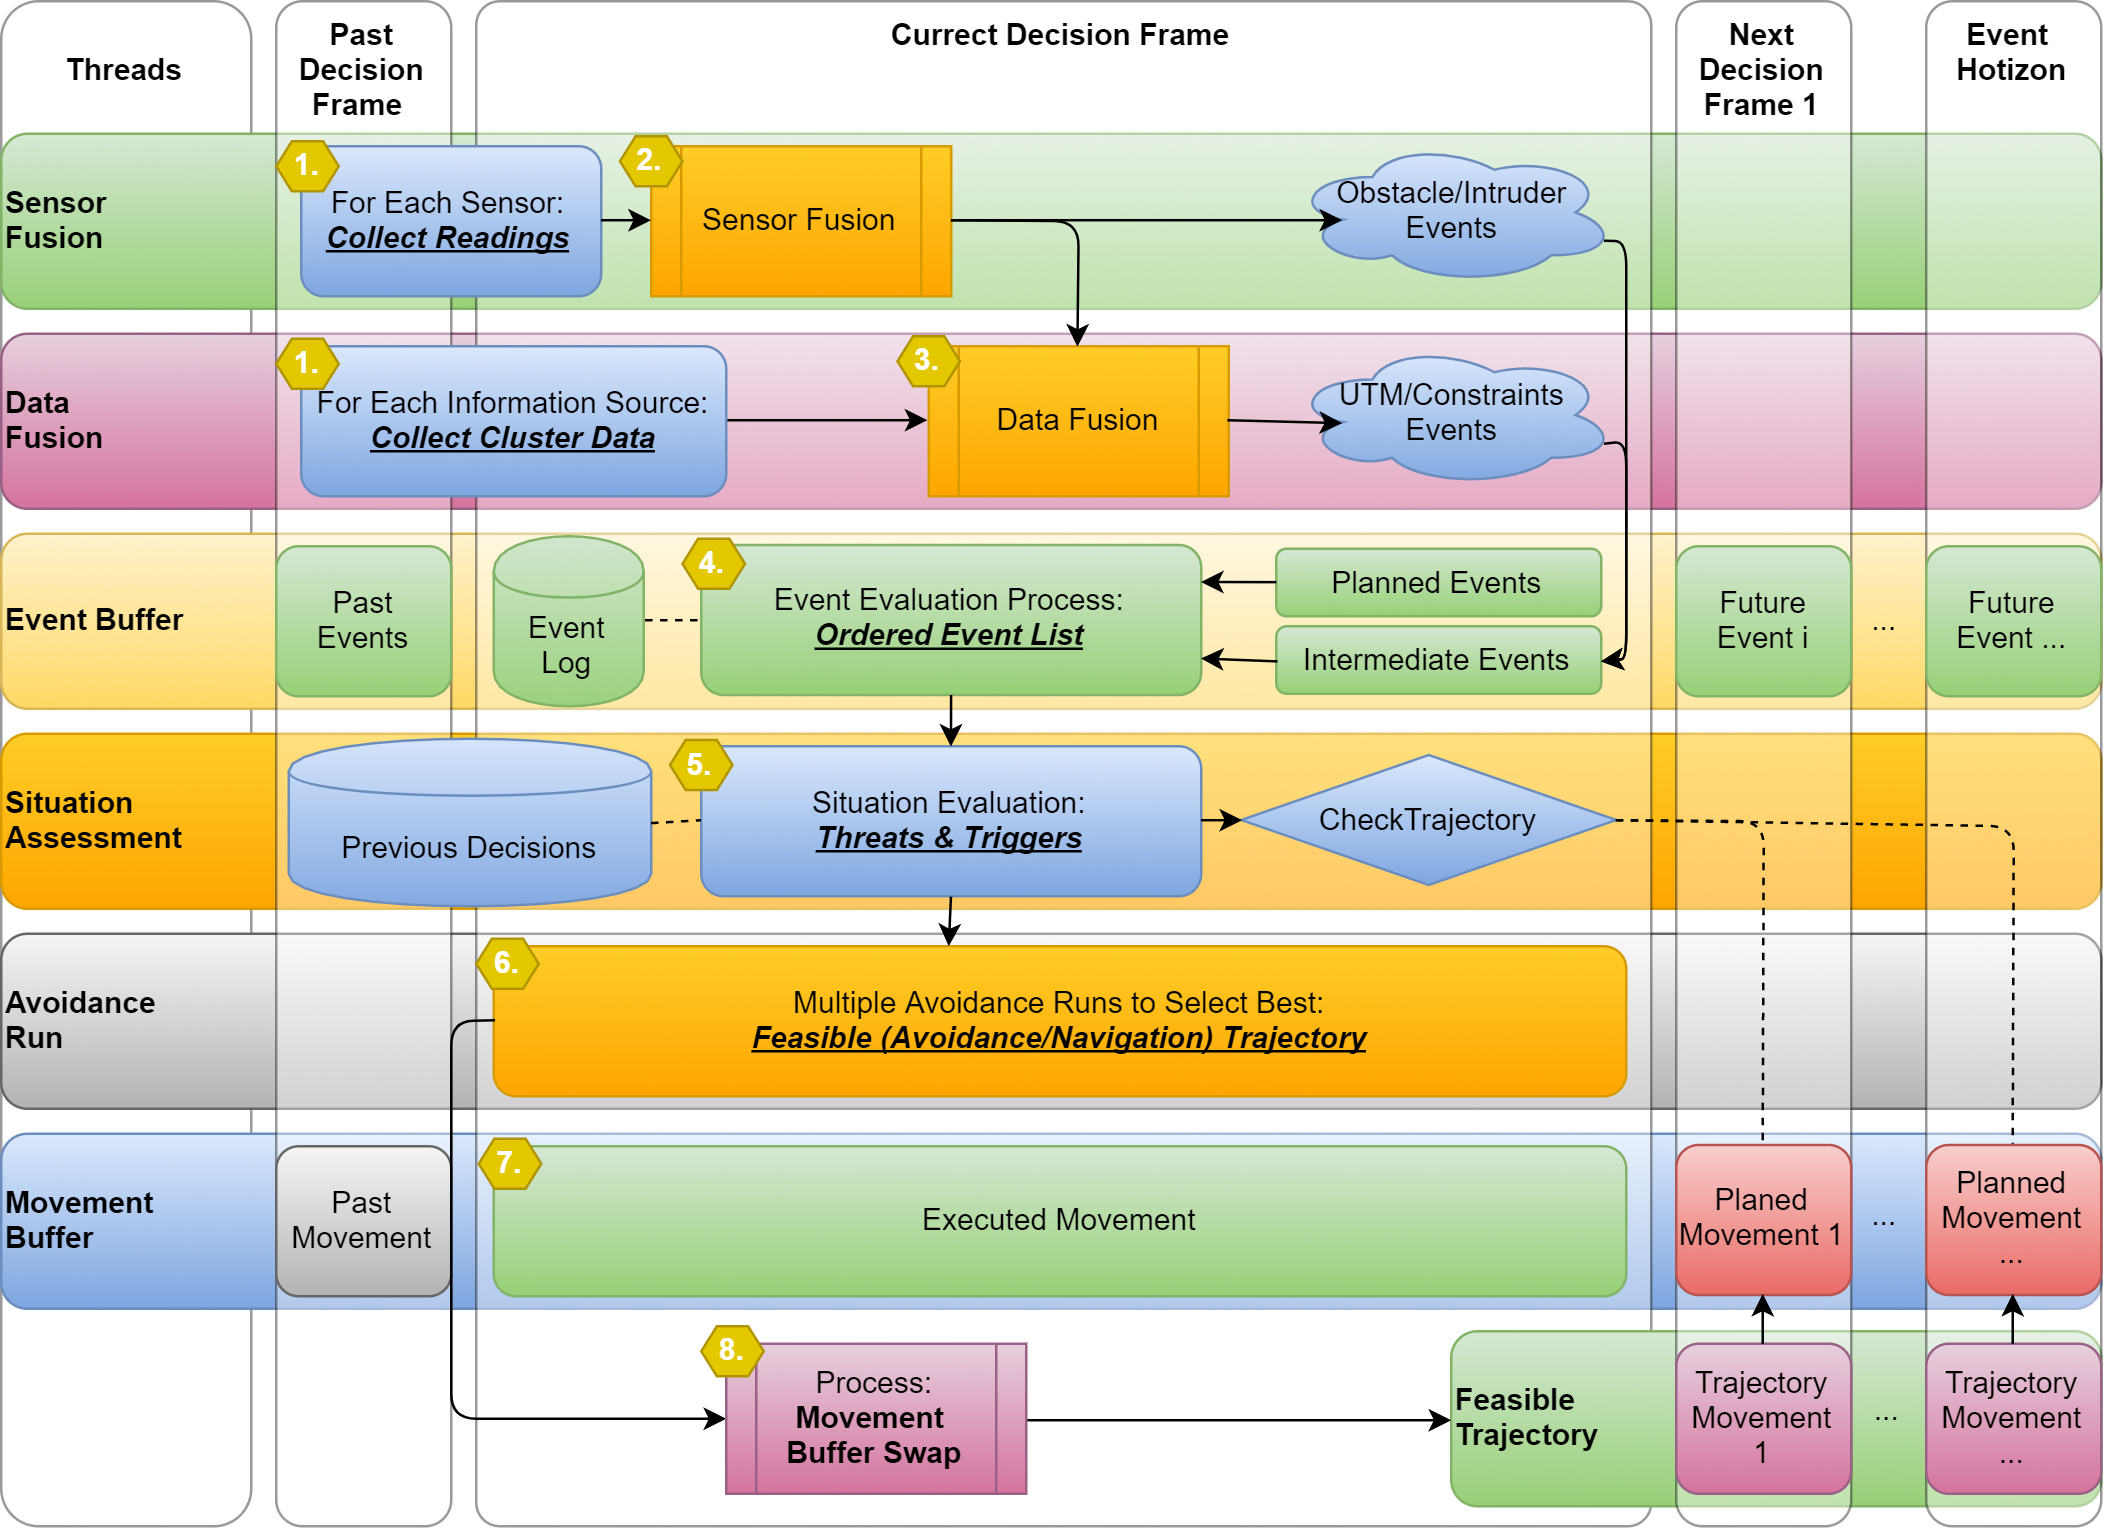
\includegraphics[width=\linewidth]{\FIGDIR/TE064DecisonFrameExplained}
    \caption{Mission control orchestration diagram.}
    \label{fig:misisonControlRunOrchestrationDiagram}
\end{figure}

    \item[3.] \emph{Event Buffer} -  special data structure to store, raise, handle, prioritize events raised by other threads. 
    
    The \emph{implemented events} are listed in 5\textsuperscript{th}-6\textsuperscript{th} step of \emph{mission control run}. The events can be categorized like follow:
    \begin{itemize}
        \item[a.] \emph{Planned events} - raised in previous decision frames to be executed in actual or future \emph{decision frame}. 
        
        \item[b.] \emph{Intermediate events} - raised in \emph{actual decision frame} by other threads to be solved intermediate. 
    \end{itemize}
    
    The event buffer thread executes following event-related activities:
    \begin{itemize}
        \item[a.] \emph{Storing} - the \emph{events} are stored in \emph{event log}. The trace is useful for process and rule fine-tuning. 
        
        \item[b.] \emph{Raising} - the combination of events (multiple avoidance events) (example sec. \ref{s:testRuleMixed}) can trigger additional avoidance behaviour in form of combined-event.
        
        \item[c.] \emph{Handling} - the events are handled by invoking the \emph{situation assessment} or by rule engine invocation (sec. \ref{s:RuleEngineArchitecture}).
        
        \item[d.] \emph{Prioritizing} - the multiple events can be risen during one \emph{decision frame}. Some events cannot be merged and needs to have proper prioritization before handling, like the \emph{obstacle detection} events before \emph{intruder detection event}.
    \end{itemize}
    
    \item[4.] \emph{Situation Assessment} - invoked by \emph{event buffer} o assess situation, responsible for proper \emph{avoidance run} (sec. \ref{s:aviudabceGridRun}) dataset preparation and invocation. The main responsibility is to check \emph{planned trajectory feasibility} stored in \emph{movement buffer} as \emph{planned movements}.
    
    \item[5.] \emph{Avoidance Run} - invoked by \emph{necessity to plan trajectory} originating from \emph{event buffer} or \emph{situation assessment} threads. The avoidance run produces one or multiple \emph{avoidance/navigation} feasible trajectories according to  7\textsuperscript{th}-11\textsuperscript{th} step of \emph{mission control run}.
    
    \item[6.] \emph{Movement Buffer} - represents \emph{movement automaton implementation} (sec. \ref{s:movementAutomatonDefinition}). The movement automaton consumes \emph{movement automaton buffer} each decision frame contains exactly one \emph{movement}. The movements can be viewed as:
    \begin{itemize}
        \item[a.] \emph{Past movements} - already executed movements in \emph{past decision frames}.
        
        \item[b.] \emph{Executed movement} - actually executed movement in current decision frame, this movement cannot be changed.
        
        \item[c.] \emph{Future movements} - future planned movements to be executed after \emph{current decision frame} expires. These movements outlines planned trajectory (predictor mode sec. \ref{s:referenceTrajectoryGenerator}).
    \end{itemize}
    
    \item[7.] \emph{Feasible Trajectory} - consists of \emph{future planned movements} taking place directly after \emph{correct decision frame}. If its necessary, the planned trajectory in movement buffer is no longer feasible, the planned movements will throw away and replaced by \emph{trajectory movements}. 
\end{itemize}

\noindent The \emph{roles \& responsibilities} of each thread have been explained to outline their orchestration and roles in \emph{mission control run} (fig. \ref{fig:missionControlRunActivityDiagram}). The numbered steps in (fig. \ref{fig:misisonControlRunOrchestrationDiagram}) shows the threads orchestration in following manner:

\begin{itemize}
    \item[1.] \emph{Sensor \& Data fusion data set preparation/collection} - the sensor readings are collected through multiple past and over current \emph{decision frame}. Each sensor reading is filtered and processed according to best practices. 
    
    The raw information from various data sources is loaded for relevant space clusters. The relevant space clusters are determined based on \emph{UAS expected position}. 
    
    \item[2.] \emph{Sensor fusion} - the readings from sensors are preprocessed according to (sec. \ref{s:staticObstacles}, \ref{s:intruders}).
    
    \item[3.] \emph{Data fusion} - the information sources are preprocessed according to (sec. \ref{s:staticObstacles}, \ref{s:intruders}).
    
    \item[4.] \emph{Event evaluation process} - the events are evaluated, if there is any triggering event (5\textsuperscript{th}-6\textsuperscript{th} mission control run steps) the situation evaluation process is called.
    
    \item[5.] \emph{Situation evaluation process} - the situation is evaluated according to 5\textsuperscript{th}-6\textsuperscript{th} mission control run steps.
    
    \item[6.] \emph{Feasible trajectory selection process} - from collected \emph{navigation/avoidance trajectories} (7\textsuperscript{th}-10\textsuperscript{th} mission control run steps). If there are more feasible trajectories (increasing threat) the one compliant with the most of the threats is selected.
    
    \item[7.] \emph{Movement execution} - the movement for \emph{current decision frame} is being executed.
    
    \item[8.] \emph{Movement buffer swap} - if there is a new \emph{feasible trajectory} the future movements for next decision frames are flushed away. The movement buffer is then filled with \emph{feasible trajectory movements}.
    \begin{note}
        This step impacts the duration of future \emph{decision frames}.
    \end{note}
\end{itemize}

    	\newpage
\subsection{\secState{R}Computation Complexity}\label{sec:MCRcomputationalComplexity}
\paragraph{Introduction:}The \emph{Computation Complexity} one mission control run assessment is necessary to identify the strong and weak points of approach. Lets get through modules to assess notable calculations/algorithms complexity on high abstraction level.

\paragraph{Navigation Loop:} I the navigation loop, the \emph{waypoint reach condition} (eq. \ref{eq:waypointReachCondition}) is checked, this is unitary operation with worst complexity $\mathscr{O}(1)$. The selection process of the next \emph{Goal Waypoint} can get through all waypoints in the mission if they are all unreachable the complexity is $\mathscr{O}(|waypoints|)$.

The \emph{notable steps} complexity is following:
\begin{equation*}
    \begin{aligned}
        \texttt{Reach Condition: }& \mathscr{O}(1)\\
        \texttt{Select Next Waypoint: }&\mathscr{O}(|waypoints|)
    \end{aligned}
\end{equation*}

\paragraph{Data Fusion:} The \emph{data fusion} is all about \emph{threat selection}. 

If \emph{UAS} is in \emph{controlled airspace} it needs to iterate over received \emph{collision Cases} to select \emph{active ones}. The complexity of this step is linear, therefore boundary is given as $\mathscr{O} (|collision Cases|)$.

Thresholding \emph{Detected Obstacles} is done by simple comparison of \emph{LiDAR ray hits} in given $cell_{i,j,k}$ of \emph{Avoidance Grid}.

Any loading of \emph{threats} from \emph{information sources} is depending on clustering. The \emph{Airspace Clustering} is considered as static for our setup. Therefore the \emph{count of active airspace clusters} has main impact on complexity. The \emph{count of information sources} is static and not changing over mission time. Information sources usually implement \emph{Hash search function} with complexity $\mathscr{O}\ln|searched Item Set|$.

\noindent The \emph{computation complexity} boundaries for \emph{Data fusion} in  our setup are following:
\begin{equation*}
    \begin{aligned}
        \texttt{Select Active Collision Cases: }& \mathscr{O} (|collision Cases|)\\
        \texttt{Threshold Detected Obstacles: }& \mathscr{O}(|cells|)\\
        \texttt{Load Map Obstacles: }& \mathscr{O}(\ln|activeClusters|\times|information Sources|)\\
        \texttt{Load Hard Constraints: }& \mathscr{O}(\ln|activeClusters|\times|information Sources|)\\
        \texttt{Load Soft Constraints: }& \mathscr{O}(\ln|activeClusters|\times|information Sources|)
    \end{aligned}
\end{equation*}

\begin{note}
    The \emph{real-time clustering} is \emph{hard non-polynomial problem} \cite{kleinberg1998microeconomic}.  Usually all information sources and sensor have \emph{polynomial complexity} of processing. The \emph{controlled airspace clusters} are usually set for very long period of time. Therefore \emph{Obstacle Map}, \emph{Airspace Constraints}, and, \emph{Weather Constraints} can be considered as preprocessed
\end{note}

\newpage
\paragraph{Situation Assessment:} The \emph{Situation Assessment} is evaluating triggering events. The \emph{evaluation} is usually simple existence question without further calculations. The \emph{complexity} of \emph{event evaluation} for our case is $\mathscr{O}(1)$. There are 8 triggers. The count of \emph{triggers} needs to be accounted in complexity boundary:

\begin{equation*}
    \mathscr{O}(|triggers|\times event Evaluation Complexity)    
\end{equation*}

\begin{note} The \emph{trigger calculation complexity} needs to stay low, because the \emph{triggers} are verified every \emph{Mission Control Run}. The \emph{Avoidance Run} trigger frequency should be very low under normal conditions.  
\end{note}


\paragraph{Avoidance Run:} The \emph{Avoidance run} is most critical part of \emph{Mission Control Run}, because \emph{Avoidance Path} calculation. The \emph{Navigation Path} calculation is less complex (Rule engine is not accounted), therefore \emph{Emergency Avoidance Mode} is assumed. 

The \emph{threat insertion} is realized in 7\textsuperscript{th} to 10\textsuperscript{th} step. The first is \emph{Avoidance Grid} filled with \emph{Static Obstacles}. The \emph{Avoidance Grid} is designed to separate rotary  \emph{LiDAR} ray space into hit count even cells. Insertion of \emph{LiDAR} scan into \emph{Avoidance Grid} complexity depends on \emph{total cell count}. The \emph{upper boundary} for \emph{insert obstacles} is given like follow:

\begin{equation*}
    \texttt{Insert Obstacles: } \mathscr{O}(|cells|)
\end{equation*}

\noindent The \emph{intruders intersection model} type impact the insertion complexity. The \emph{linear intersection} (sec. \ref{s:linearIntersectionModel}) is going through maximum of \emph{layers count} cells. 

The \emph{body volume intersection model} (sec. \ref{s:bodyvolumeIntersection}) can check the \emph{simple intersection condition} over all \emph{Avoidance Grid} in worst case, therefore complexity for this check is bounded by \emph{count of cells}. 

The \emph{Maneuverability Uncertainty Intersection} (sec. \ref{s:uncertaintyIntersection}) can hit all cells in \emph{Avoidance Grid}. The calculation complexity boundary is exponential depending on \emph{horizontal/vertical} spread in $[rad]$. The \emph{intersection} implementation was done \emph{ad-hoc}. The impact of \emph{intersection application} is visible only when there is more than \emph{4} concurrence intruders (fig. \ref{fig:emergencyHeadOnMultipleComputationTime}).

\noindent The \emph{complexity boundary for \emph{intruder insertion}} is given like follow:

\begin{equation*}
    \texttt{Insert Intruders: }
    \mathscr{O}\left(\sum \begin{bmatrix}
        |linear Intersections| \times |layers|\\
        |body volume Intersections| \times  |cells|\\
        |cells|^{horizontal Spread \times vertical Spread}\\
    \end{bmatrix}\right)
\end{equation*}

\begin{note}
    The \emph{intruder intersection} is critical in \emph{non-controlled airspace}. The main complexity gain in \emph{controlled airspace} is from \emph{rule application}. Our \emph{rule complexity} is in worst case depending on \emph{Reach Set} node count and \emph{Active Collision Cases} count.
    
    \begin{equation*}
        \texttt{Apply Our Rules: } \mathscr{O}(|active Collision Cases| \times |nodes|)
    \end{equation*}
\end{note}

\newpage\noindent For \emph{Hard/Soft Constraints} The algorithm used for intersection polygons was selected based on study \citep{bentley1979algorithms}, the selected algorithm  \emph{Shamos-Hoey} \cite{shamos1976geometric}. The \emph{calculation complexity} boundary is given like follow:

\begin{multline*}
    \texttt{Hard Constraints Intersection:}\\ \mathscr{O}(|cells|\times|hard Constraints| \times \max |constraint Points|^2)
\end{multline*}
\begin{multline*}
    \texttt{Soft Constraints Intersection:}\\ \mathscr{O}(|cells|\times|soft Constraints| \times \max |constraint Points|^2)
\end{multline*}

\noindent Each \emph{threat} category application in \emph{Mission Control Run} is done after \emph{each intersection} in 7\textsuperscript{th} to 10\textsuperscript{th} step. All ratings (tab. \ref{tab:defuzificationRatings}) expect $Reachibility(cell_{ij,k})$ and $Reachibility(Trajectory)$  are calculated. The \emph{calculation complexity} boundary for one \emph{reachibility rating} is $\mathscr{O}(1)$. (eq. \ref{eq:trajectoryReachibility}, \ref{eq:cellReachibility}). The \emph{Recalculate Reachibility} operation applied $4\times$ have maximal \emph{complexity} boundary given as follow:

\begin{equation*}
    \texttt{Recalculate Reachibility: } \mathscr{O}(4 \times (|nodes| + |cells|))
\end{equation*}

\noindent Each time at the end of in 7\textsuperscript{th} to 10\textsuperscript{th} step the \emph{Avoidance Path is Selected}. The \emph{Worst Case} (expected) scenario is to \emph{select} four paths for each \emph{treath} application. The algorithm for \emph{best path selection} (alg. \ref{alg:FindBestPathAvoidanceGrid}) iterates over all \emph{cells} in avoidance grid and over all \emph{trajectories} passing through that cell. The complexity boundary for \emph{path selection} is given as follow:

\begin{equation*}
    \texttt{Select Path: } \mathscr{O}\left(4 \times \left(|cells|+\frac{|nodes|}{|cells|}\right)\right)
\end{equation*}


\paragraph{Conclusion:}  Overall approach complexity is \emph{low}. If proper \emph{Information Sources} with efficient clustering and \emph{intersection models for intruders} are used, the approach will stay within \emph{non-polynomial complexity}. 
The average load time for \emph{testing scenarios} is summarized in (tab. \ref{tab:computationLoadStatistics}).

\begin{note}
    The calculation of \emph{Reach Set} is eliminated by pre-calculation for \emph{state range} \cite{gomola2017obstacle}.
\end{note}
 

%% This adds a line for the Bibliography in the Table of Contents.
\addcontentsline{toc}{chapter}{Bibliography}
%% *** Set the bibliography style. ***
%% (change according to your preference/requirements)
%\bibliographystyle{plain}
%% *** Set the bibliography file. ***
%% ("thesis.bib" by default; change as needed)
\bibliography{thesis}

%% *** NOTE ***
%% If you don't use bibliography files, comment out the previous line
%% and use \begin{thebibliography}...\end{thebibliography}.  (In that
%% case, you should probably put the bibliography in a separate file and
%% `\include' or `\input' it here).

\end{document}
